\RequirePackage{lineno}

\documentclass[cits]{JINST}
%%\usepackage{multirow}
\usepackage{times}
%%\usepackage{hyperref}
\usepackage{lineno}
\usepackage{amsmath, amsthm, amssymb}
\usepackage{mathptmx}
\usepackage{mdwlist}
\usepackage{textcomp}
\usepackage{graphicx,subfigure}
\usepackage{fontenc}
%%\usepackage{color}

\title{Measuring directionality in double-beta decay and neutrino interactions with kiloton-scale scintillation detectors}

\author{C.~Aberle$^a$, A.~Elagin$^b$, H.J.~Frisch$^b$, M.~Wetstein$^b$, and L.~Winslow$^a$\setcounter{footnote}{0}\thanks{corresponding author}\\
\llap{$^a$}University of California, Los Angeles, Los Angeles, CA 90095, USA\\
\llap{$^b$}University of Chicago, Chicago, IL 60637, USA\\
  E-mail: \email{lwinslow@physics.ucla.edu}}

\linenumbers

\abstract{Large liquid-scintillator-based detectors have proven to be
exceptionally effective for low energy neutrino measurements due to
their good energy resolution and scalability to large volumes. The
addition of directional information using Cherenkov light and fast
timing would enhance the scientific reach of these detectors,
especially for searches for neutrino-less double-beta decay. In this
paper, we develop a technique for extracting particle direction using
the difference in arrival times for Cherenkov and scintillation light,
and evaluate several detector advances in timing, photodetector
spectral response, and scintillator emission spectra that could be
used to make direction reconstruction a reality in a kiloton-scale
detector.}

\keywords{Scintillators, scintillation and light emission processes (solid, gas and liquid scintillators); Cherenkov detectors; Large detector systems for particle and astroparticle physics; Neutrino detectors; Simulation methods and programs}

\newcommand{\nuebar}{$\overline{\nu}_{e}$}
\newcommand{\PerTonDay}{(ton$\cdot$day)$^{-1}$}
\newcommand{\GEANT}{GEANT4}
\newcommand{\RCS}{$R_{C/S}$}
\hyphenation{KamLAND}


\begin{document}

\section{Introduction}
Liquid scintillator-based detectors are responsible for several of the
critical measurements that have determined our present understanding
of neutrino masses and mixings. These measurements include KamLAND's
measurement of reactor anti-neutrino oscillation at a distance of
$\sim$200~km\cite{kam2013}, Borexino's measurement of $^{7}$Be solar
neutrino oscillation\cite{borexino}, and most recently the short
baseline reactor anti-neutrino experiments that measured oscillations
due to $\theta_{13}$ at a distance of 1~km: Daya Bay\cite{dbtwo},
Double Chooz\cite{dctwo, dchydrogen}, and RENO\cite{reno}.
Scintillator-based neutrino detectors will continue to be important for the
next set of neutrino measurements, from the determination of the
neutrino mass hierarchy\cite{juno,reno50} to elastic scattering
measurements\cite{isodarscatt} and sterile neutrino
searches\cite{isodar,nist}, and for non-proliferation
applications\cite{nucifer, songs}.

The scalability of these detectors to large volumes also makes them
highly competitive for neutrino-less double-beta ($0\nu\beta\beta$)
decay searches in which the final state consists of a pair of
electrons with energies in the few MeV range.  The observation of this
rare decay would prove that the neutrino is a Majorana particle, which
would have profound consequences to our understanding of the generation of
mass and may provide a possible explanation of the matter-antimatter
asymmetry in the universe.  Currently one of the best limits for the
$0\nu\beta\beta$ half-life comes from the scintillating detector
KamLAND-Zen\cite{KZ0nu}.

The advantage of liquid scintillators for measurements in the
$\sim$1~MeV range is their scalability from 1~ton to 1~kiloton while
providing energy resolutions of $\sim$5\%. This is roughly a factor of
two better than water Cherenkov detectors, the other developed
technology that can be economically scaled to these large
masses. However, for scintillator-based detectors, while the energy
resolution is good due to the abundance of light, the light is
isotropic and does not retain the directional information of the
primary particle.  In contrast, the direction of the particle can be
reconstructed from the Cherenkov cone in water-based detectors,
although the energy resolution rapidly degrades below $\sim$5~MeV. For
double-beta decay in particular, but also for neutrino interactions,
the directional information can be a strong suppressant of
backgrounds.

In a liquid-scintillation-based detector, Cherenkov light is also
produced, although most is absorbed and re-emitted as part of the
scintillation processes.  However, some fraction retains its
directional information. If this directional Cherenkov light can be
isolated from the copious isotropic scintillation light, it may be
possible to reconstruct the direction of the primary particle or, in
the case of double-beta decay, to determine the existence and topology
of the pair.  The addition of directionality is thus a powerful tool
for background rejection.  In this paper, we develop a technique for
separating the Cherenkov and scintillation light using the photon arrival
times and evaluate several detector advances in timing, photodetector 
spectral response, and scintillator emission spectra that would allow
the realization of direction reconstruction in kilo-ton scale
scintillating neutrino detectors. This is a different technique and application than the direction reconstruction described for high-energy neutrino interactions\cite{john} or that for neutrons from inverse beta decay\cite{chooz,dcDirection}. 

\section{Liquid scintillator detectors}
Liquid scintillators are `cocktails' of aromatic hydrocarbons. When
charged particles move through a scintillator, the molecules are
excited, predominantly via the non-localized electrons in the
$\pi$-bonds of the phenyl groups\cite{birks_book}. Vibrational
and rotational modes of the molecules are turned into heat within
picoseconds through collisions with other molecules.  Within $\sim$10
picoseconds, the $\pi$-electrons de-excite to the first excited state
from higher levels through radiationless transitions. The first
excited state can de-excite through photon emission. There are two
characteristic times for this de-excitation, depending if the singlet
state or the triplet state was excited.  The singlet state will
de-excite within nanoseconds while the triplet state de-excites on the
order of 10's or 100's of nanoseconds. These two processes are
fluorescence and phosphorescence respectively. The exact time
constants for these processes are determined by the composition of the
scintillator.

The absorption and emission spectra overlap at some level
in all molecules. Consequently, if there is only one type of molecule in
the scintillator cocktail the light output is reduced due to
inefficiencies in the energy transfer through multiple absorption and
re-emission processes. Aromatic solutes or fluorophores are added to the
primary solvent to shift the wavelengths of the photons to higher values 
where the scintillator is more transparent. This
wavelength-shifting is also used to match the quantum efficiency as a
function of wavelength for the photodetectors being used. One typical
scintillator mixture uses pseudocumene as the solvent with 1-5~g/l of
PPO as the fluorophore. This mixture has a peak emission at about 400~nm
where bialkali photomultiplier tubes (PMTs) are most sensitive and the
pseudocumene is relatively transparent.

A good liquid scintillator will produce $\sim$10,000 photons
isotropically per MeV of deposited energy. Although less abundant,
Cherenkov light will be produced as well if a particle is moving
faster than the speed of light in the medium.  This light is emitted
in a cone centered on the direction of the particle trajectory, and
with a continuous spectrum weighted toward shorter wavelengths but
extending well into the red. The spectrum is described
by\cite{Cherenkov34}:
\begin{equation}
\label{eqCherenkov}
\frac{d^2N}{d\lambda dx} = \frac{2 \pi \alpha Z^2}{\lambda^2} \left [ 1 - \frac{1}{\beta^2 n(\lambda)^2} \right ]
\end{equation}
where $n(\lambda)$ is the wavelength-dependent index of refraction and
$\beta$ is the velocity of the incoming particle. In a large detector,
the Cherenkov light produced at wavelengths shorter than the
absorption cutoff of the scintillator will be absorbed and re-emitted
as isotropic light, but wavelengths longer than this cutoff will
propagate across the detector, retaining their directional
information. These undisturbed Cherenkov
photons will have timing determined by the group 
velocity\cite{group_velocity_article,pdg_review_2012,tamm1939} in the liquid,
\begin{equation}
\label{eqGroup}
v_{g}(\lambda) = \frac{c_{vacuum}}{n(\lambda) - dn(\lambda)/d\textnormal{log}(\lambda)}.
\end{equation}
The longer wavelength Cherenkov photons typically arrive before the
scintillation light, which is slowed by both the scintillation
processes and the shorter wavelengths involved. Thus, with sufficient
timing resolution and sensitivity to longer wavelengths it should be
possible to separate the directional Cherenkov light and the isotropic
scintillation light, and then to reconstruct the direction of the
initial particle.

In $0\nu\beta\beta$, the electrons emerge with a combined energy equal
to the Q-value of the particular isotope. The individual
electrons follow distributions of energies and angular correlations, 
a probable case being equal division of energy between back-to-back
electrons\cite{phasespace}. This case is shown in figure \ref{detector_view}
for an example $^{116}$Cd $0\nu\beta\beta$ event. Since the decay
half-life is inversely proportional to the phase-space factor, isotopes with
higher Q-values are preferred and due to backgrounds from the daughters
of the $^{238}$U and $^{232}$Th decay chains those with Q-values at or
above 2.6~MeV are most often considered for $0\nu\beta\beta$ searches.
There are hundreds of candidate $0\nu\beta\beta$ isotopes\cite{tabledbb},
but only a handful with large Q-values. 

Most of the high Q-value candidates
have been considered as a dopant for a liquid scintillator:
$^{150}$Nd (Q=3.367~MeV)\cite{minfang,nd1}, $^{96}$Zr (Q=3.350~MeV)\cite{zr1},
$^{100}$Mo (Q=3.034~MeV)\cite{mo1}, $^{82}$Se (Q=2.995~MeV)\cite{qdot},
$^{116}$Cd (Q=2.81~MeV)\cite{qdot, cd1}, $^{130}$Te (Q=2.533~MeV)\cite{qdot, biller},
$^{136}$Xe (Q=2.479~MeV)\cite{KZ0nu} and $^{124}$Sn (Q=2.29~MeV)\cite{sn1}.
Xenon gas readily dissolves into liquid scintillator. For the other isotopes,
a suitable organometallic compound needs to be found that produces a stable
scintillator with a long attenuation length in the wavelength region of
interest. As an alternative to single-atom-doping, recently nanocrystals 
formed by candidate isotopes have been explored as a dopant\cite{qdot,qdot2}.

\section{Geant4 simulation}
\label{sim_section}
In order to study the effects relevant to directional reconstruction
in liquid scintillators, a \GEANT \newline 
\cite{geant4one,geant4two} simulation
has been constructed. The simulation uses \GEANT~version 4.9.6 with the default liquid scintillator
optical model, in which optical photons are
assigned the group velocity in the wavelength region of normal
dispersion.

\begin{figure}
        \begin{center}
        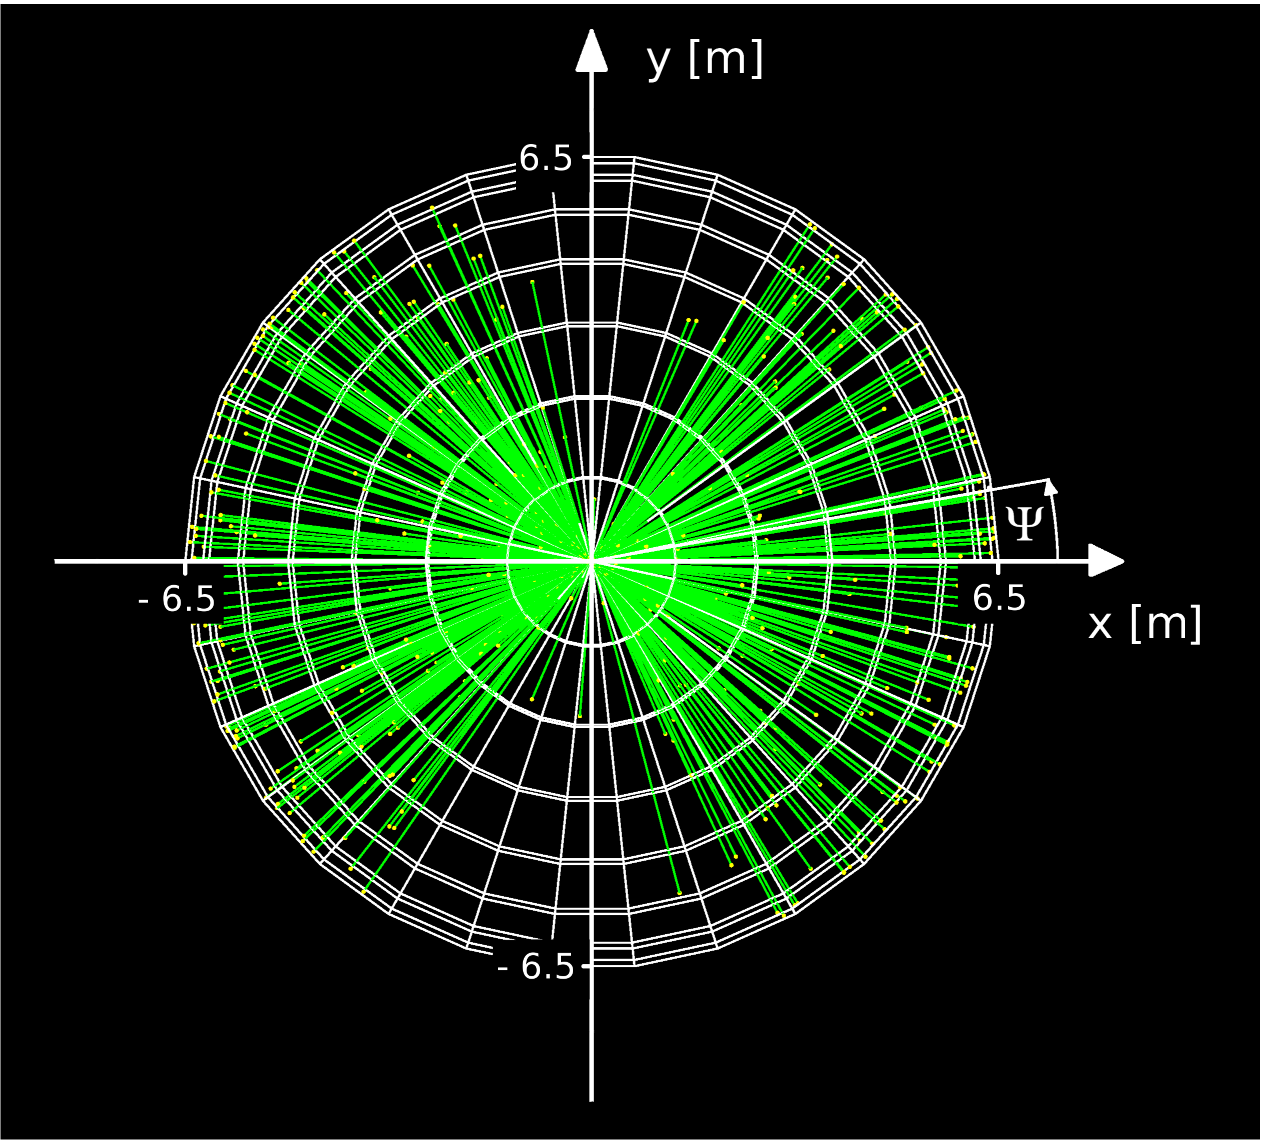
\includegraphics[scale=0.4]{graphs/geometry_plot_labels.pdf}
        \caption[]{The detector geometry and coordinate system.
        The radial rays (green lines) are photons emitted by two back-to-back electrons with 1.4~MeV each
        (equally divided energy of $^{116}$Cd~$0\nu\beta\beta$ decay). The electrons originate at
        the center of the sphere with initial directions along the x
        and -x-axis. Only Cherenkov photons are drawn to illustrate the
        directionality of the event. \label{detector_view}}
        \end{center}
\end{figure}

The detector geometry is a sphere of 6.5~m radius filled with
scintillator. Figure \ref{detector_view} shows the geometry and the
Cherenkov light from an example $^{116}$Cd $0\nu\beta\beta$ event. The
default scintillator properties have been chosen to match a KamLAND-like
scintillator\cite{kamland2003}: 80\% n-dodecane, 20\% pseudocumene
(1,2,4-trimethylbenzene) and 1.52~g/l PPO (2,5-diphenyloxazole). The
scintillator properties implemented in the simulation include the
atomic composition and density ($\rho$ = 0.78~g/ml), the
wavelength-dependent attenuation length\cite{tajimaMaster} and
refractive index\cite{OlegThesis}, the scintillation emission
spectrum\cite{tajimaMaster}, emission rise time ($\tau_r$ = 1.0~ns)
and emission decay time constants ($\tau_{d1}$ = 6.9~ns and
$\tau_{d2}$ = 8.8~ns with relative weights of 0.87 and 
0.13)\cite{tajimaThesis}, scintillator light yield (9030 photons/MeV)
and the Birks constant ($kB$ $\approx$ 0.1~mm/MeV)\cite{ChrisThesis}. 
Variations from the baseline KamLAND case are
discussed below. Re-emission of absorbed photons in the scintillator
bulk volume and scattering have not yet been included, but are not
expected to change the conclusions here.


The inner sphere surface is used as the photodetector. It is treated
as fully absorbing (no reflections), with a photodetector coverage of
100\%. Two important photodetector properties have been varied: 1)
the transit-time spread (TTS, default $\sigma$ = 0.1~ns) and 2) the
wavelength-dependent quantum efficiency (QE) for photoelectron
production. The default is the QE of a bialkali photocathode (Hamamatsu
R7081 PMT)\cite{Hamamatsu_R7081}, for which digitized values come from the Double Chooz\cite{dctwo}
Monte Carlo simulation. We note that the KamLAND 17-inch PMTs use the
same photocathode type with similar quantum efficiency.

\begin{figure}[tbh]
\begin{center}
        \subfigure[ ~Default
        simulation.]{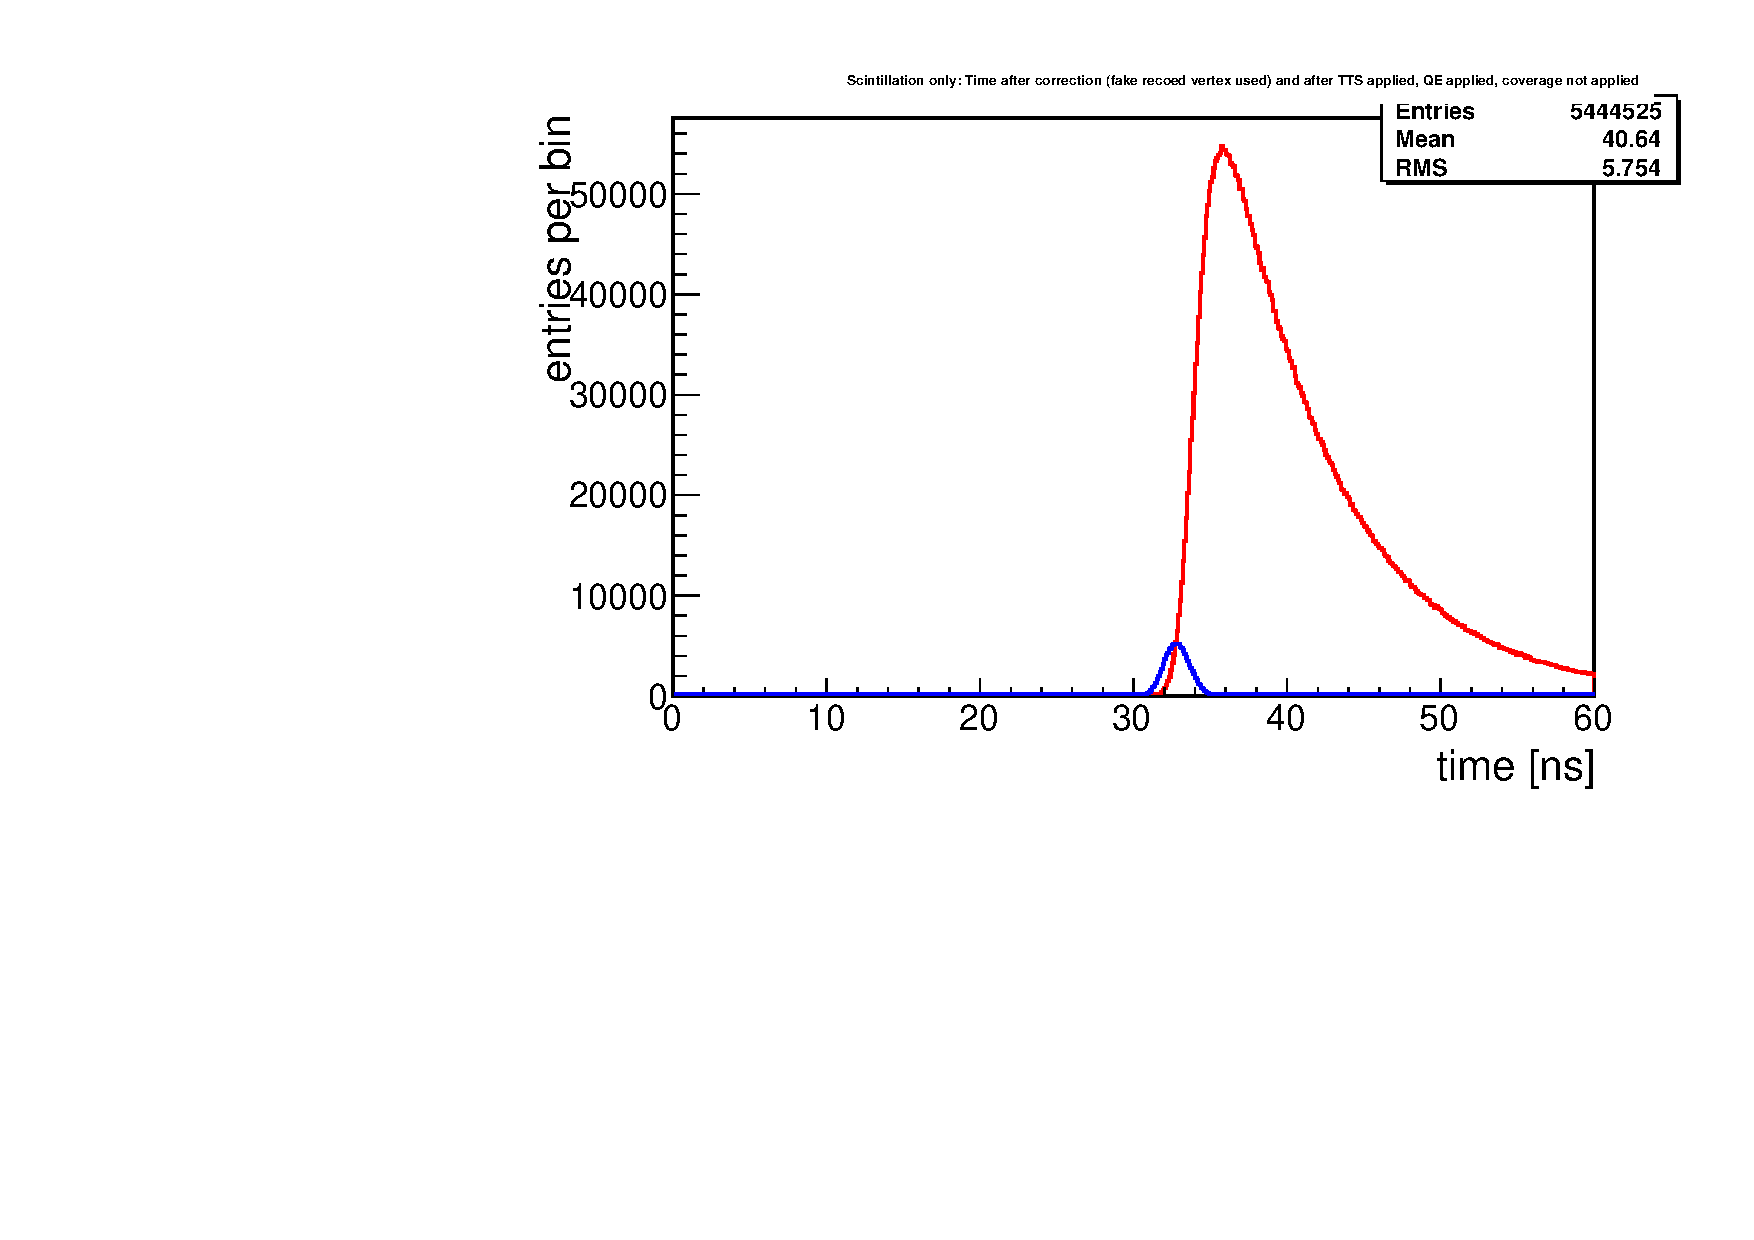
\includegraphics[scale=0.295]{graphs/6p5Meter_5MeVElectrons_Bialkali_KamlandScintSpec_TIME.pdf}}
        \subfigure[ ~Increased TTS
        (1.28~ns).]{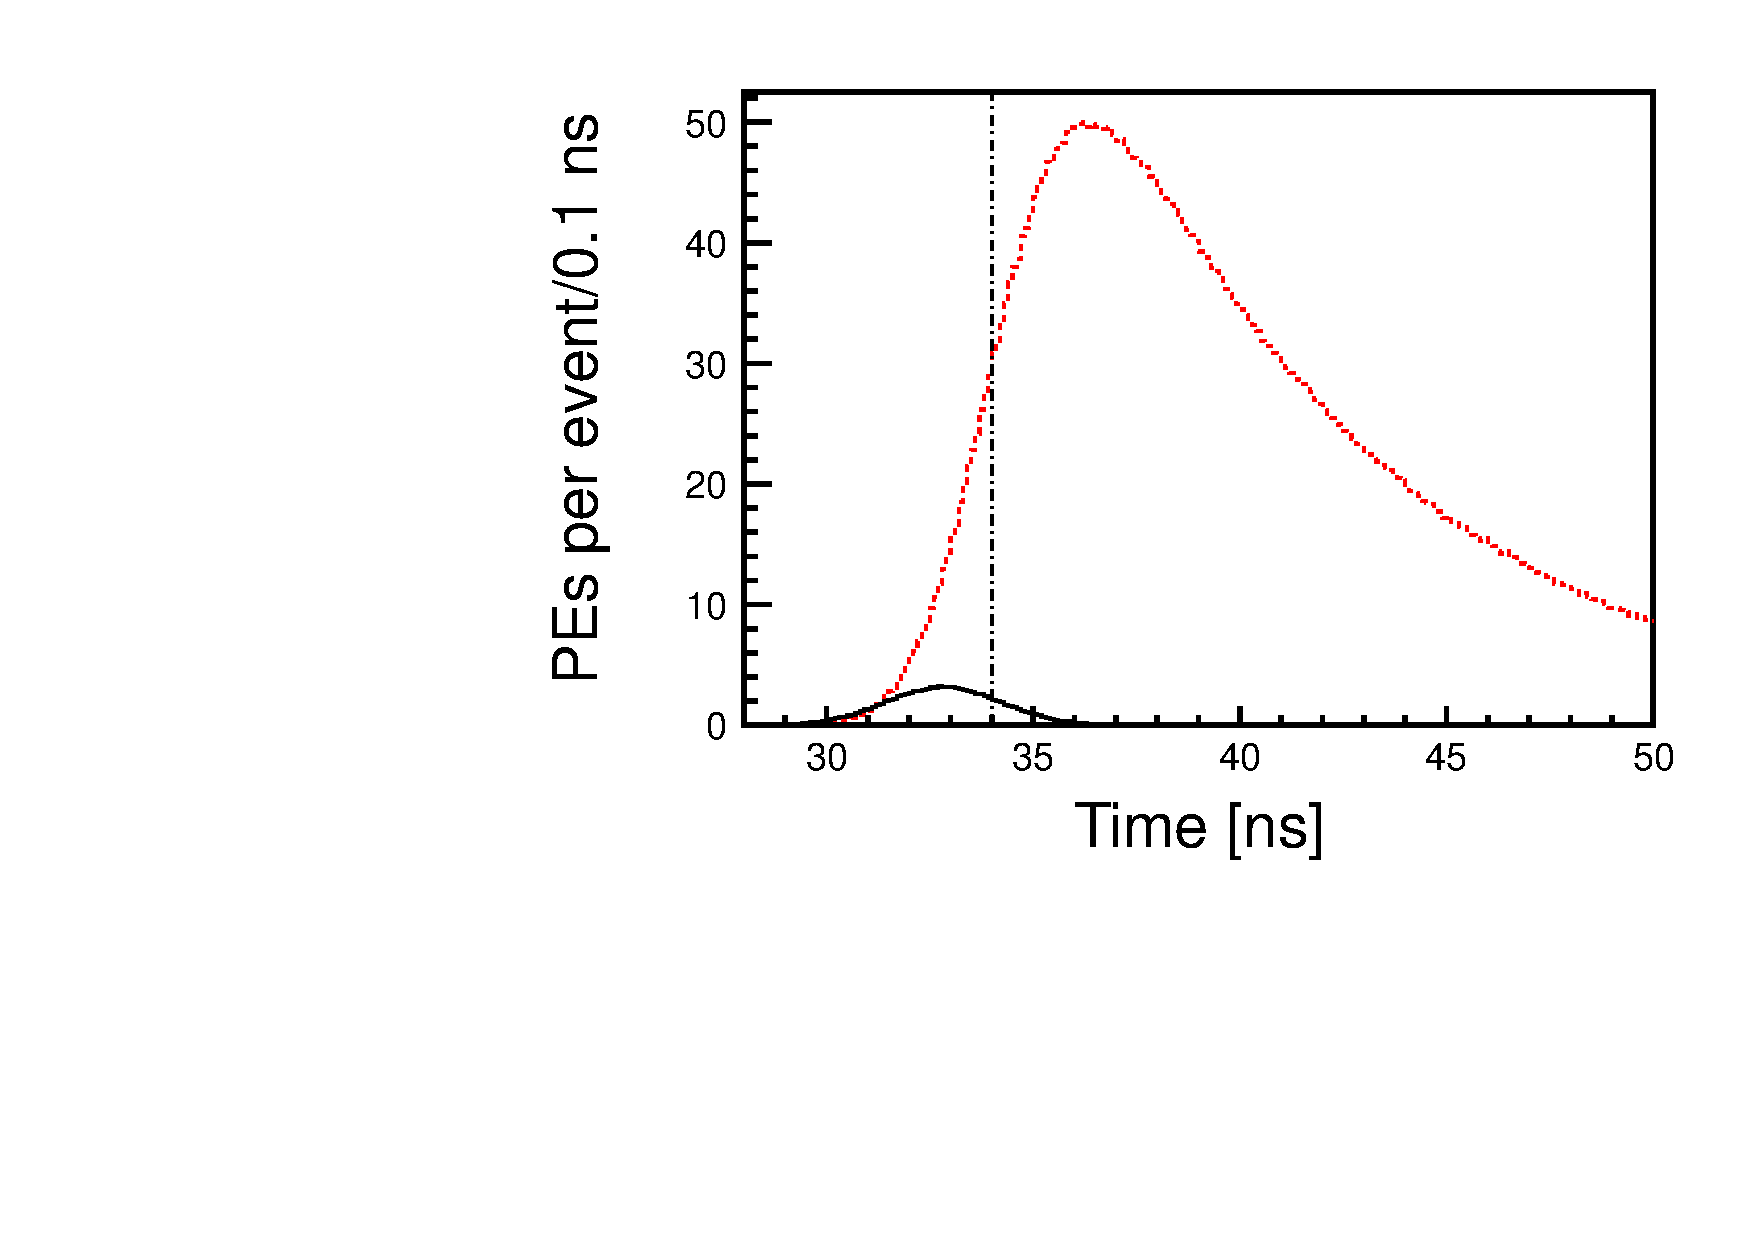
\includegraphics[scale=0.295]{graphs/6p5Meter_5MeVElectrons_Bialkali_KamlandScintSpec_1p28nsTTS_TIME.pdf}}
        \subfigure[ ~Red-sensitive
        photocathode.]{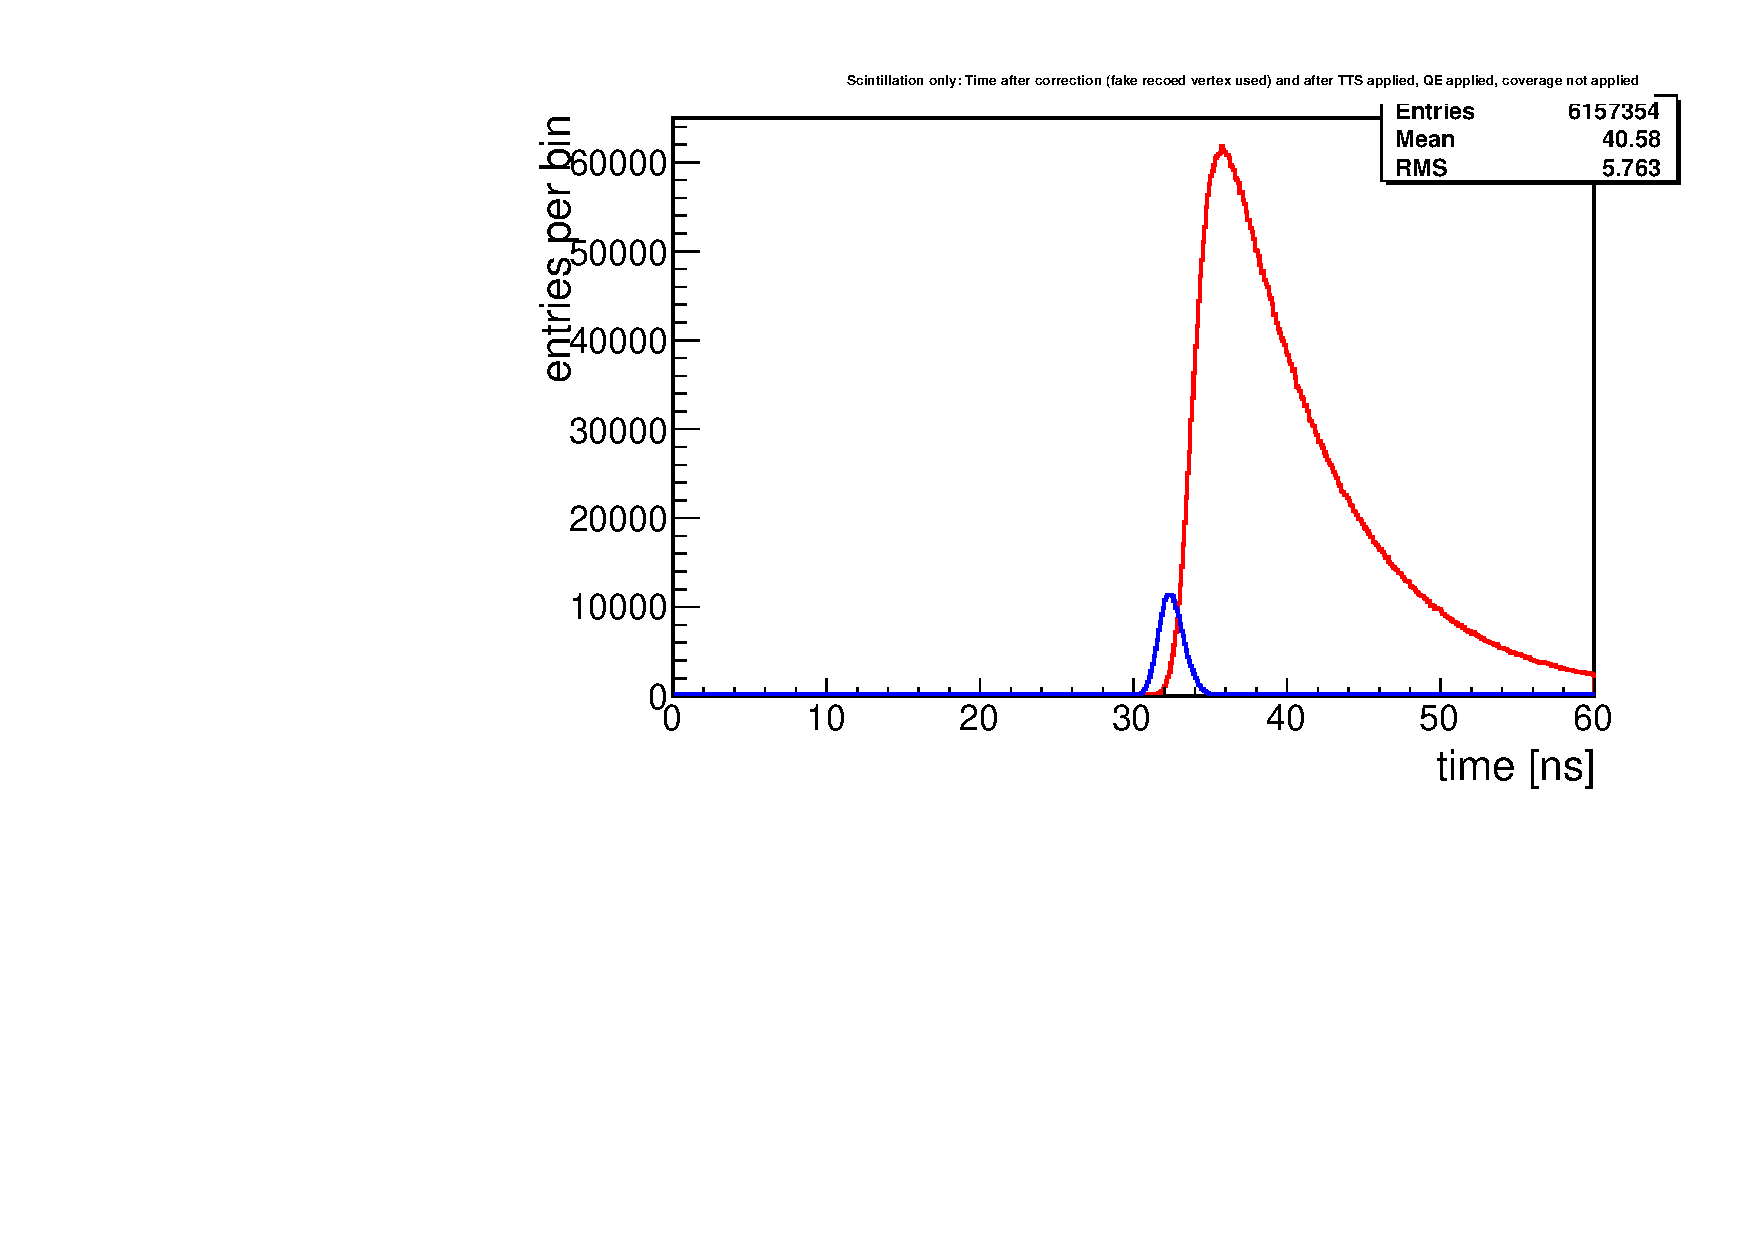
\includegraphics[scale=0.295]{graphs/6p5Meter_5MeVElectrons_RedSensitiveQE_KamlandScintSpec_TIME.pdf}}
        \caption[]{Photoelectron (PE) arrival times after application
        of the transit-time spread (TTS) for the simulation
        of 1000 electrons (5~MeV) with different values of the TTS and
        wavelength response. PEs from
        Cherenkov light (black, solid line) and scintillation light
        (red, dotted line) are
        compared. The dash-dotted vertical line illustrates a time cut at
        34.0~ns. (a) Default simulation: bialkali photocathode and TTS =
        0.1~ns ($\sigma$). After the 34.0~ns time cut we get 171~PEs
        from scintillation and 108~PEs from Cherenkov light. (b)
        Default simulation settings except for TTS = 1.28~ns (KamLAND
        17 in. PMTs). After the 34.0~ns time cut we get 349~PEs from
        scintillation and 88~PEs from Cherenkov light. (c) Default
        simulation settings except for a GaAsP photocathode. After the
        34.0~ns time cut we get 226~PEs from scintillation and 229~PEs
        from Cherenkov light. \label{time_plots_comparison}}
        \end{center}
\end{figure}

The studies in sections \ref{sim_section} to \ref{reconstruction_sec} are made with single 5~MeV electrons, lower energies are
discussed in section \ref{edep_section}. Future studies will work on increasing the complexity
of the event as is needed for $0\nu\beta\beta$ studies. Three
effects primarily contribute to the timing of the scintillator detector
system. First, the simulated travel time of the initial 5~MeV electron is typically between
0.10 and 0.15~ns, while the travel distance is about 3~cm. Second, the
scintillation light emission follows a distribution characterized by
scintillator-specific rise and decay times. Before the solutes in
liquid scintillator can emit optical photons, the energy has to be
transferred from the solvent to the solute. The time constant of this
energy transfer accounts for a rise time in scintillation light
emission. Past neutrino experiments were not highly sensitive to the
effect of the scintillation rise time, which is the reason why there
is a lack of accurate numbers. We assume a rise time of 1.0~ns; more
detailed studies are needed in the future. The two time constants used
to describe the falling edge of the scintillator emission time
distribution (quoted above) are values specific to the KamLAND
scintillator. Third, chromatic dispersion turns out to be an important
effect in a 6.5m-radius detector at the level of precision needed for
direction reconstruction.

Due to the wavelength-dependence of the refractive index the speed of
light in the scintillator (see Equation (\ref{eqGroup})) increases
with increasing photon wavelengths for normal dispersion, with red
light traveling faster than blue light.  In order to study the
measurability of the time differences, we simulated 5~MeV electrons at
the center of the sphere where we used instantaneous scintillation
emission with the quantum-efficiency applied, but not including a
transit-time spread. The true hit time distributions of photoelectrons
were analyzed for scintillation light and Cherenkov light
separately. Photoelectrons coming from Cherenkov light are on average
created about 0.5~ns earlier than PEs from scintillation light. The
RMS values from PE time distributions for Cherenkov and scintillation
light are both about 0.5~ns. Note that these numbers include the
effect of the finite electron travel time.

The measurement of the arrival times of single photoelectrons is
affected by the transit-time spread (TTS) of the photodetectors, a
number which can be different by orders of magnitude depending on the
detector type. The default TTS of 0.1~ns ($\sigma$) is a value which
can be achieved with the large area picosecond photodetectors
(LAPPDs)\cite{LAPPDSum,LAPPDTDR} and possibly hybrid photodetectors
(HPDs)\cite{hpdThesis}; even significantly lower TTS numbers are
realistic with the LAPPD\cite{RSI_paper,PSEC4_paper,anode_paper}. We
note that uncertainties in the vertex reconstruction will produce a
similar effect to the smearing due to the TTS.

In Sections \ref{detector_timing_sec} to
\ref{scintillator_emission_sec}, we study the
photoelectron timing for different detector configurations. We focus
on the idea of increasing the discrimination between Cherenkov and
scintillation light by using improved detector timing. The primary
quantities provided by the \GEANT~simulation are the photoelectron hit
positions and the detection times after the TTS resolution has been
applied. In Section~\ref{reconstruction_sec} these quantities are then
used for event reconstruction.

\section{Detector timing}
\label{detector_timing_sec}

We first discuss results for the default simulation settings described
in the previous section. Figure \ref{time_plots_comparison} (a) shows
the TTS-smeared photoelectron (PE) detection times for 1000 simulated
electrons with 5~MeV energy in the center of the detector, with initial
momentum directions coinciding with the x-axis. The photoelectrons
induced by Cherenkov light arrive earlier, as expected due to the
instantaneous emission and the higher average photon speed compared to
scintillation light. There is, however, significant overlap of the two
arrival time distributions.

In order to compare simulations with different parameters, a fixed
time cut of $t\leq$ 34.0~ns is applied using the truth information to
isolate the Cherenkov light in this early time window. For the default
simulation case, the average number of PEs per event coming from
Cherenkov light in the early time window (108) is 98\% of the total
average number of PEs from Cherenkov light (110). For scintillation
light, the average number of PEs (171) is only 3.1\% of the average total
scintillation-induced PEs (5445). This demonstrates the effectiveness of
a time cut to separate Cherenkov light from scintillation light. 

The ratio of Cherenkov-induced to scintillation-induced photoelectrons
in the early time window ($R_{C/S}$) is a useful figure-of-merit when
comparing different simulation settings, since a higher ratio means
more directional information per PE. For the default simulation
settings $R_{C/S}=0.63$.

\begin{figure}
        \begin{center}
        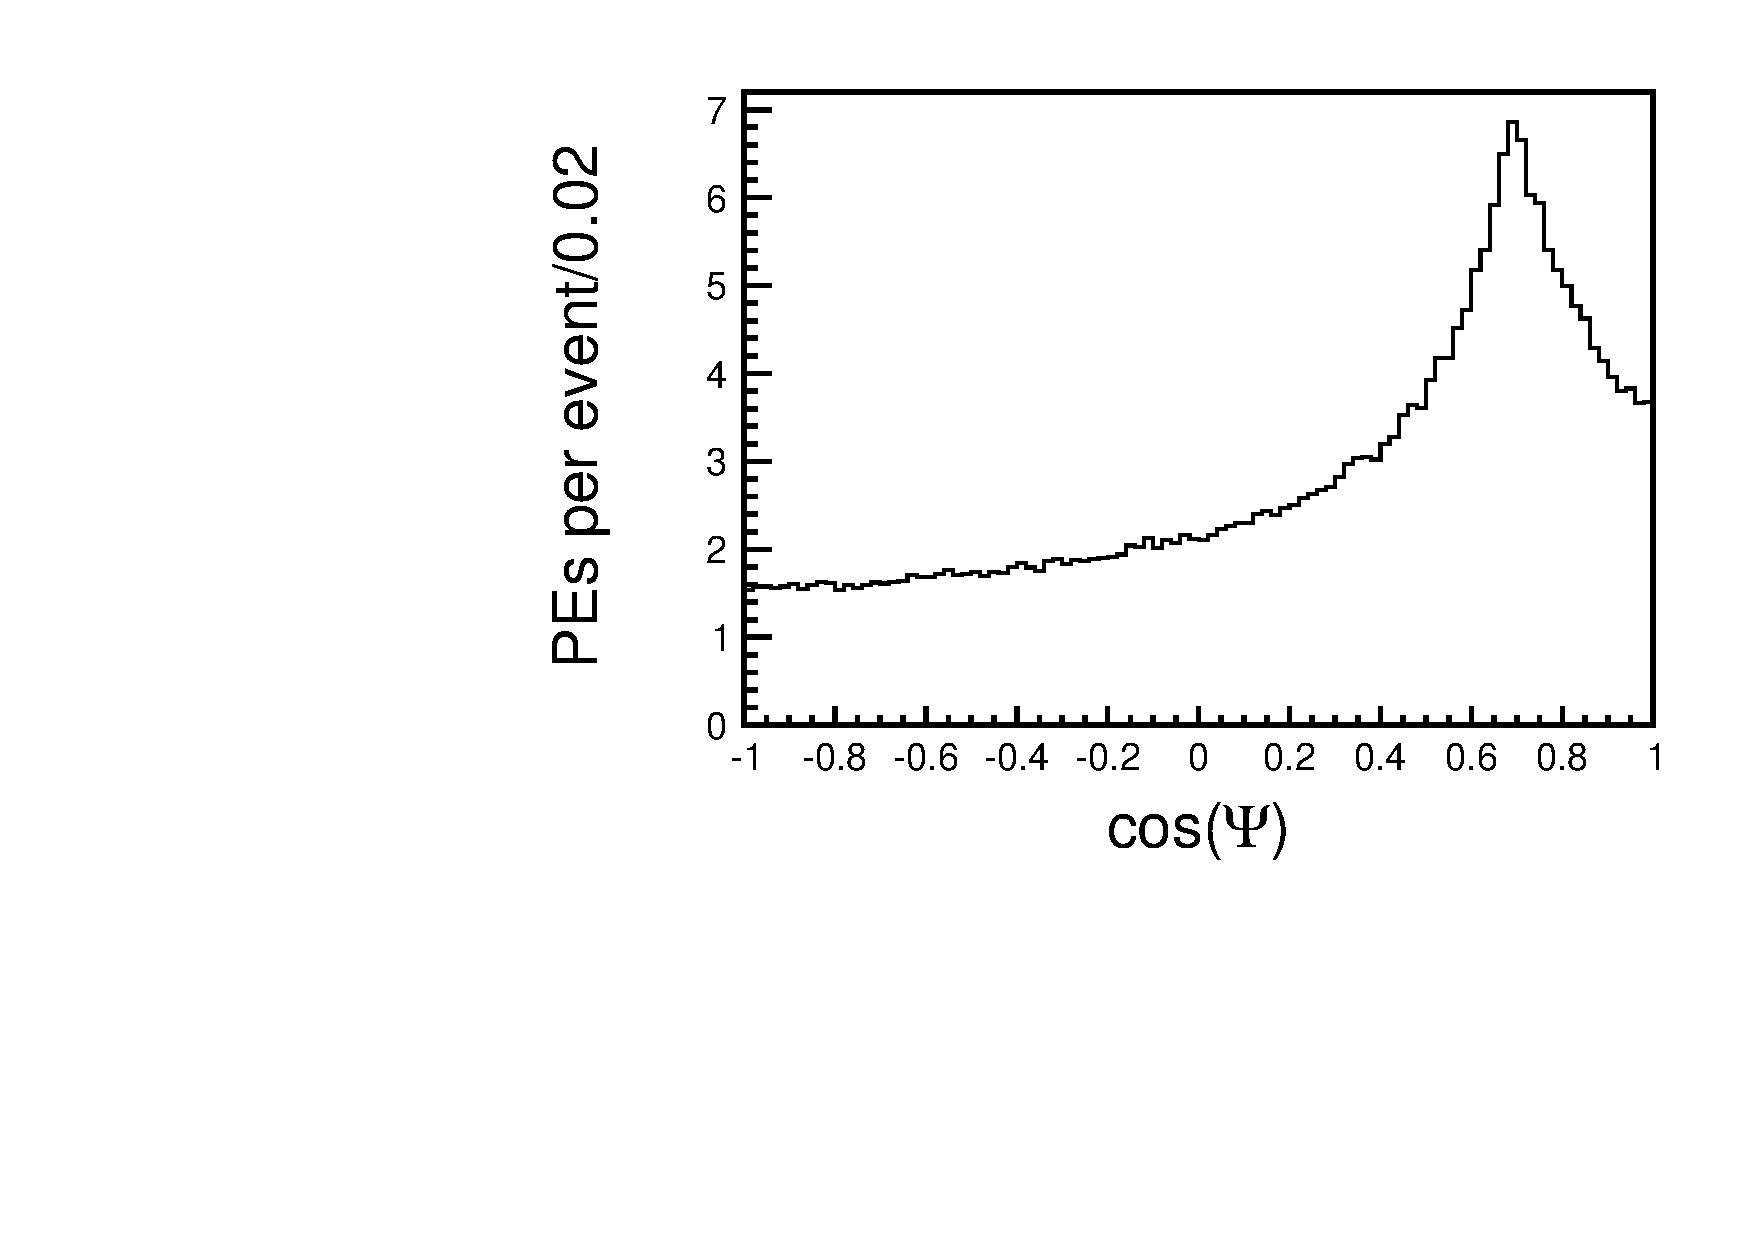
\includegraphics[scale=0.40]{graphs/cos_psi_34_h.pdf}
        \caption[]{The angular distribution of photoelectron hits
        relative to the original electron direction, $\cos(\Psi) =
        x_{hit}/|\vec{r}_{hit}|$. The sample consists of 1000 events
        with a 5~MeV electron produced at the detector center. Default
        simulation settings are used and both Cherenkov and
        scintillation light are included. The $t\leq$ 34.0~ns cut is applied.} 
        \label{Cherenkov_cone}
        \end{center}
\end{figure}

Figure \ref{Cherenkov_cone} displays the angular distribution of PE
hits after the time cut. Although this time cut is a simplification of actual time
reconstruction effects, we can use it to indicate the spatial
distribution of hits in the early time window. The Cherenkov ring structure
can be clearly seen in the peak near 46\textdegree, demonstrating
that the directional signal conveyed by the Cherenkov photons is not
erased by scattering of the initial 5~MeV electrons.

When the 17-inch KamLAND PMTs\cite{tajimaMaster,kume_1983} (TTS =
1.28~ns) are used in the simulation, the broadening of the time
distributions leads to a strongly decreased ratio of Cherenkov over
scintillation light ($R_{C/S}=0.25$) for $t<34.0$~ns (see
figure \ref{time_plots_comparison} (b)). This shows that a low
photodetector TTS is critical for directionality reconstruction and
motivates the use of novel photodetector types.

\section{Detector wavelength response}
\label{detector_wavelength_response_sec} 
In addition to decreasing the photodetector TTS to enhance $R_{C/S}$,
it is possible to optimize the wavelength-dependence of the
photocathode. Since Cherenkov photons which pass through meters of
scintillator have on average longer wavelengths than scintillation
photons, a photodetector which is more sensitive at long wavelengths
increases not only the absolute number of PEs but also the ratio
between Cherenkov- and scintillation-induced PEs.

We have run the simulation with the QE of an extended red-sensitive
GaAsP photocathode (Hamamatsu R3809U-63)\cite{Hamamatsu_R3899U}.
Figure \ref{time_plots_comparison}(c) shows the results for the
modified simulation with high QE in the red spectral region. The
higher absolute number of photoelectrons coming from Cherenkov light
(factor of $\approx$ 2) and the increased Cherenkov/scintillation
ratio ($R_{C/S}=1.01$) in the early time window would significantly improve the
directionality reconstruction.

\section{Scintillator emission spectrum}
\label{scintillator_emission_sec}
An alternative route towards increasing the separation in time between
Cherenkov and scintillation photon hits is the tuning of the
scintillator emission spectrum. Recently, the use of quantum dots
(QDs) in liquid scintillators has been studied as a possibility to
improve future large scale neutrino experiments\cite{qdot,qdot2}. One
major motivation for quantum-dot-doped scintillator is control of the
emission spectra by tuning the size or composition of the quantum
dots; quantum dots can also provide a mechanism for introducing an 
isotope for studying double-beta decay.  

The emission spectrum of commercial alloyed core/shell
CdS$_x$Se$_{1-x}$/ZnS quantum dots was measured in
Ref.\cite{qdot2}. This spectrum shows a symmetric peak centered
around 461~nm with FWHM = 29~nm.  In order to isolate the effect of
the different emission spectrum, the other simulation settings,
including the KamLAND absorption spectrum, were kept unchanged; we
find $R_{C/S}=0.17$ for the default 34.0~ns timing cut.  Compared to
the default case shown in figure \ref{time_plots_comparison}(a) the
separation is worse (as expected) because the scintillation light
wavelengths are longer than in the KamLAND emission spectrum.

However, advances in the production of commercial quantum dot samples
could yield quantum dots which have similar, single peak emission
shapes at lower wavelengths. This case has been simulated using the
same spectral shape of the measured core-shell quantum dot emission
but shifted to lower wavelengths such that the emission peak is
centered at 384~nm. This peak emission value has been measured for
other types of QDs, however with a much more pronounced 
tail\cite{qdot2}. The resulting PE time distribution shows improved
separation of Cherenkov and scintillation light compared to the
default simulation. After the 34.0~ns cut on the TTS-smeared PE time
we obtain a Cherenkov/scintillation ratio of $R_{C/S}=0.86$ (107 PE
from Cherenkov light and 124 PE from scintillation). The number of
Cherenkov-induced PEs after the time cut is unchanged while the number
of PEs coming from scintillation light is decreased due to the higher
average photon travel times.
\begin{figure}[tbh]
        \begin{center}
        %%\subfigure{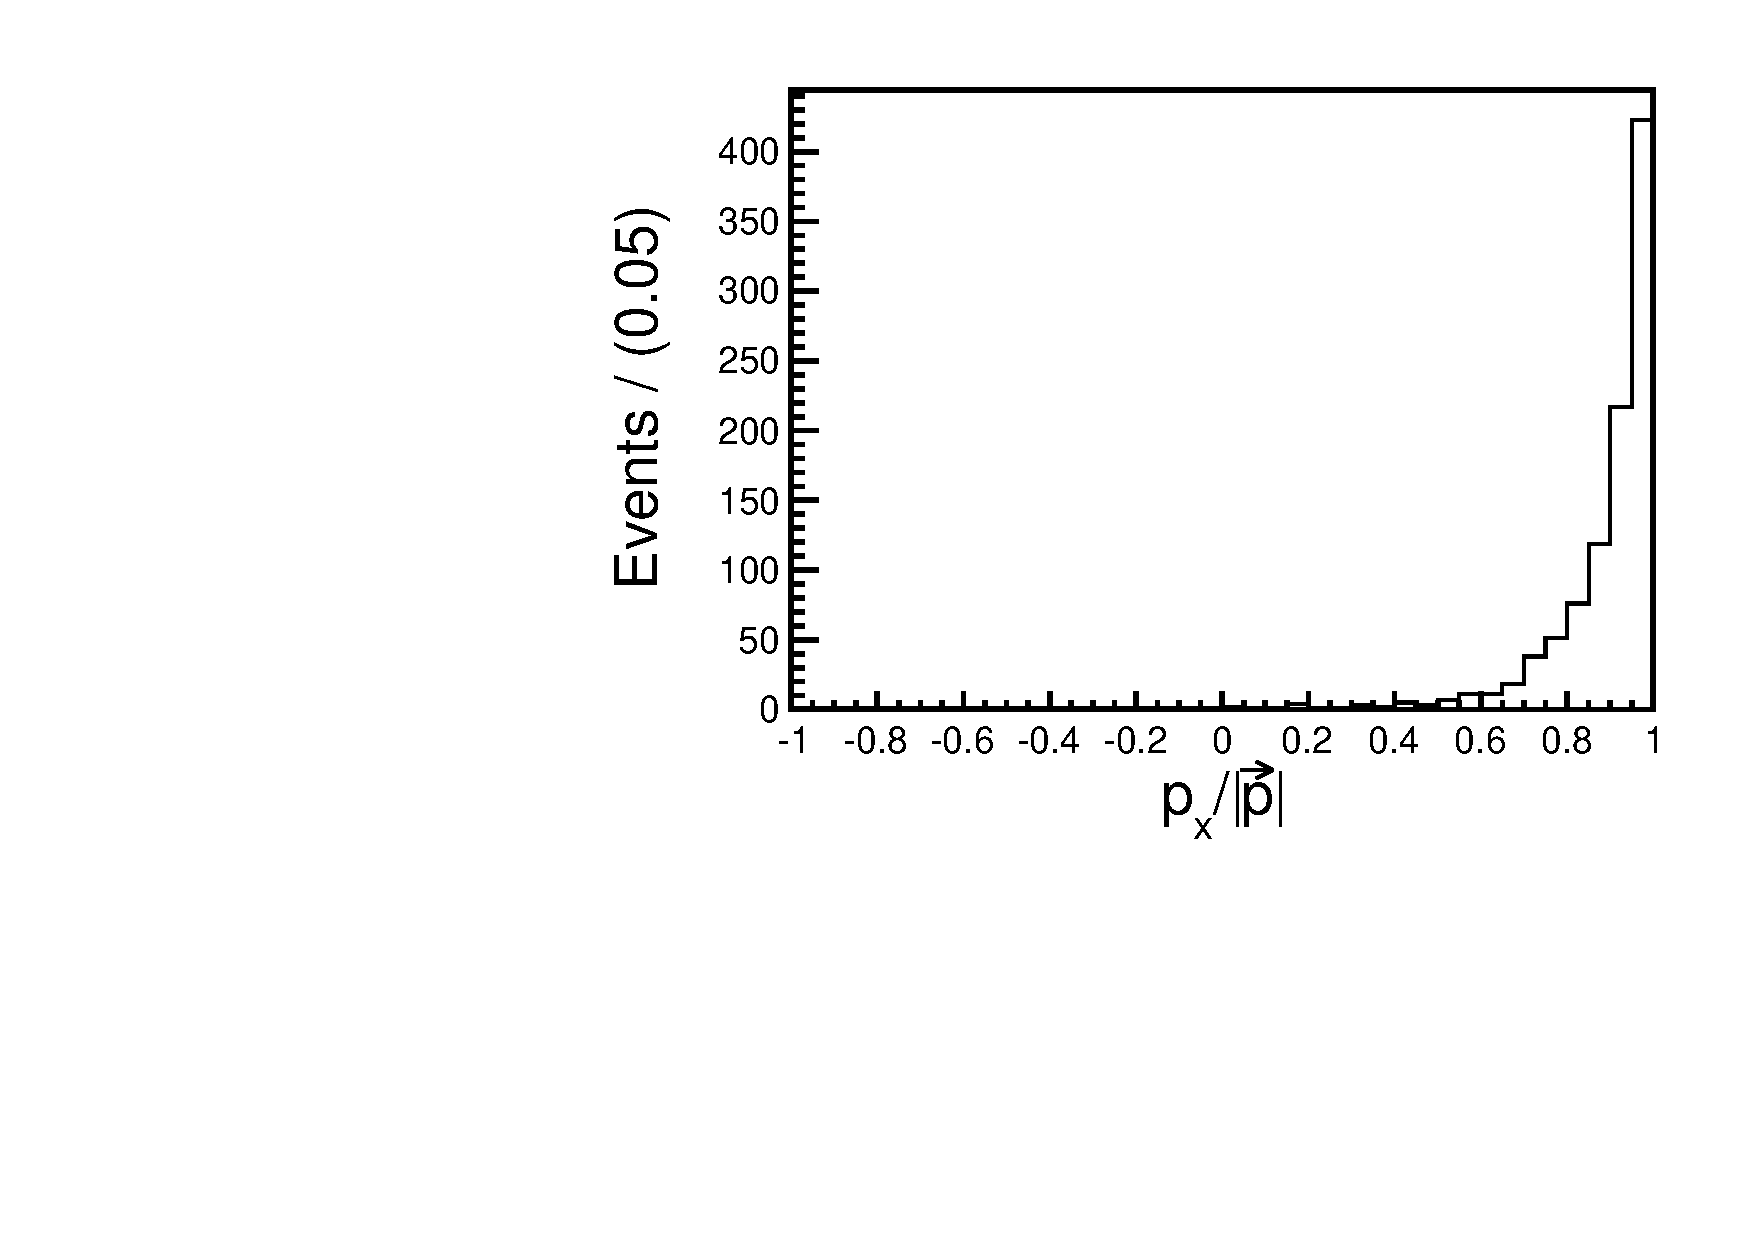
\includegraphics[scale=0.295]{graphs/hDirX_v1.pdf}}
        %%\subfigure{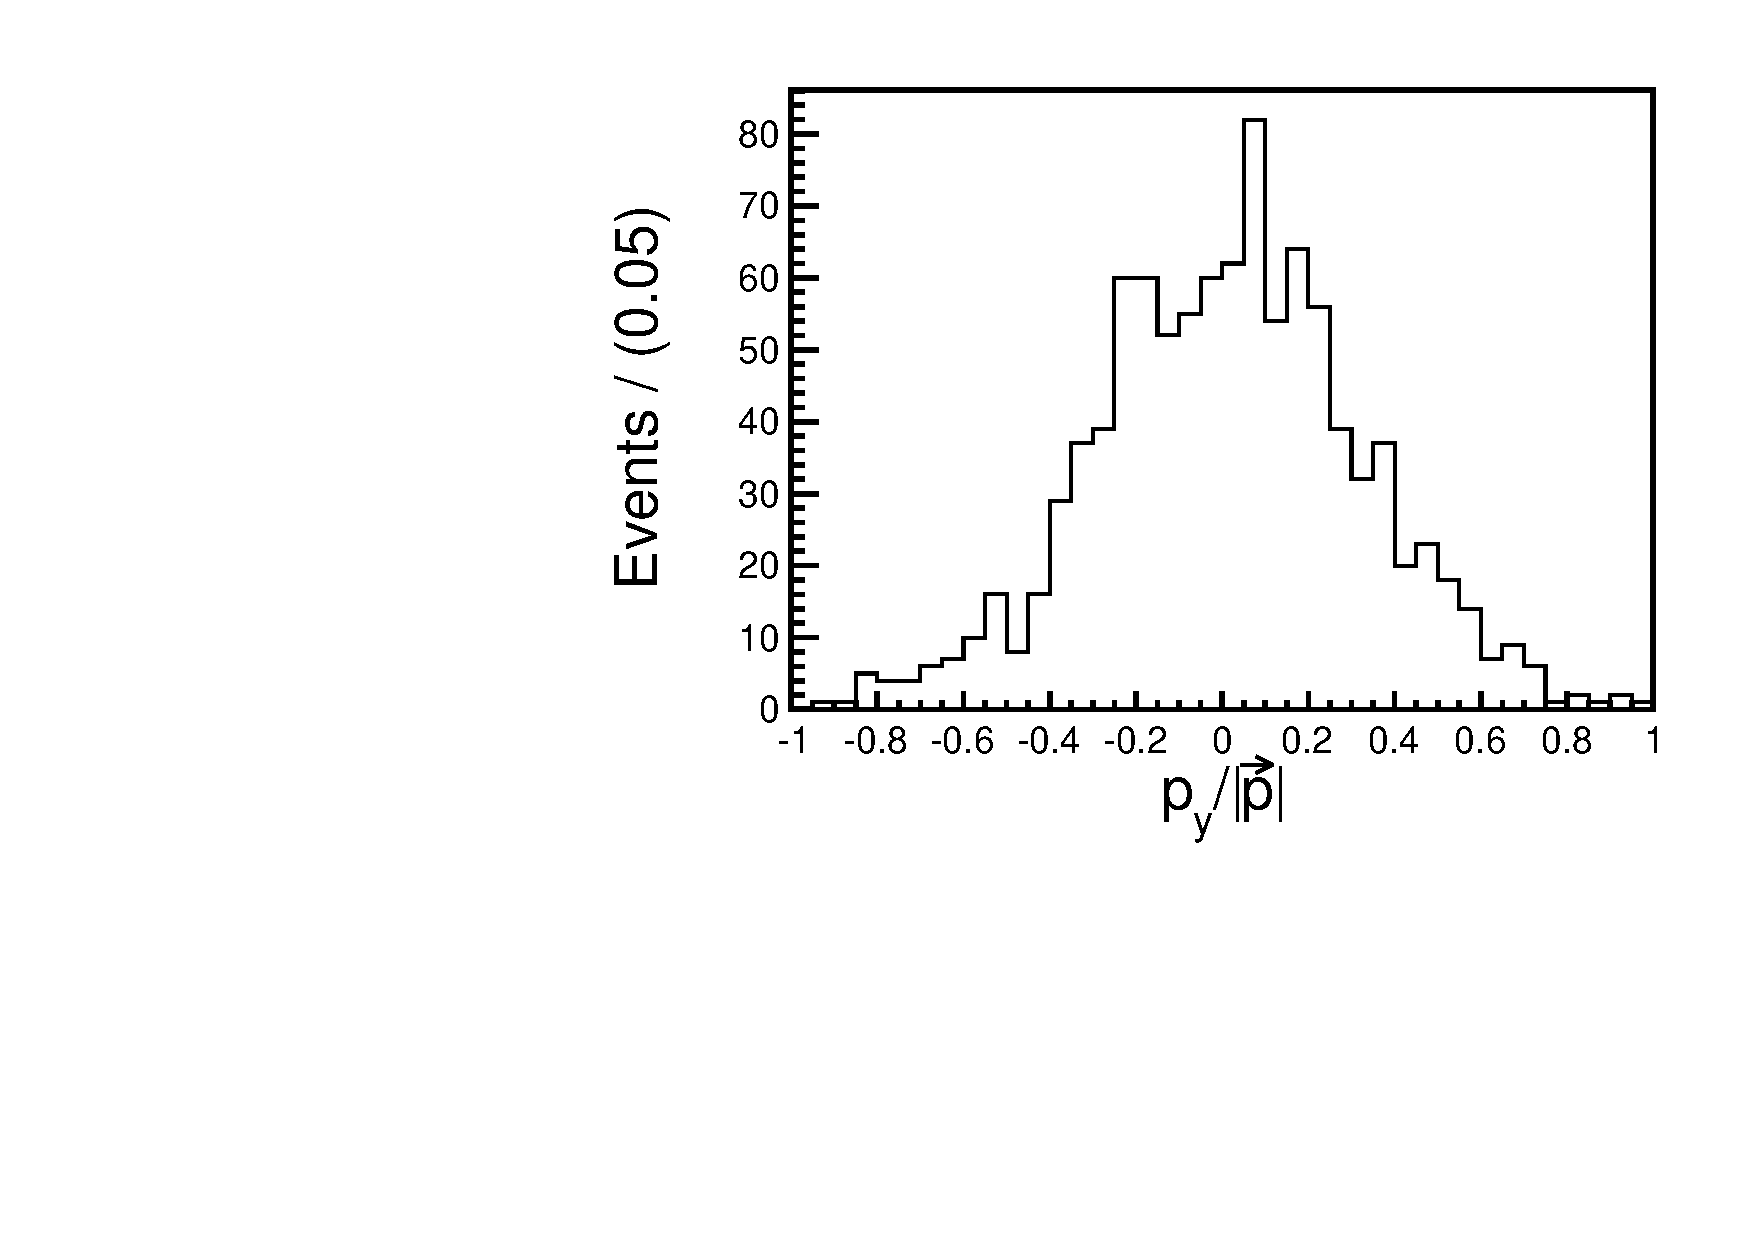
\includegraphics[scale=0.295]{graphs/hDirY_v1.pdf}}
        %%\subfigure{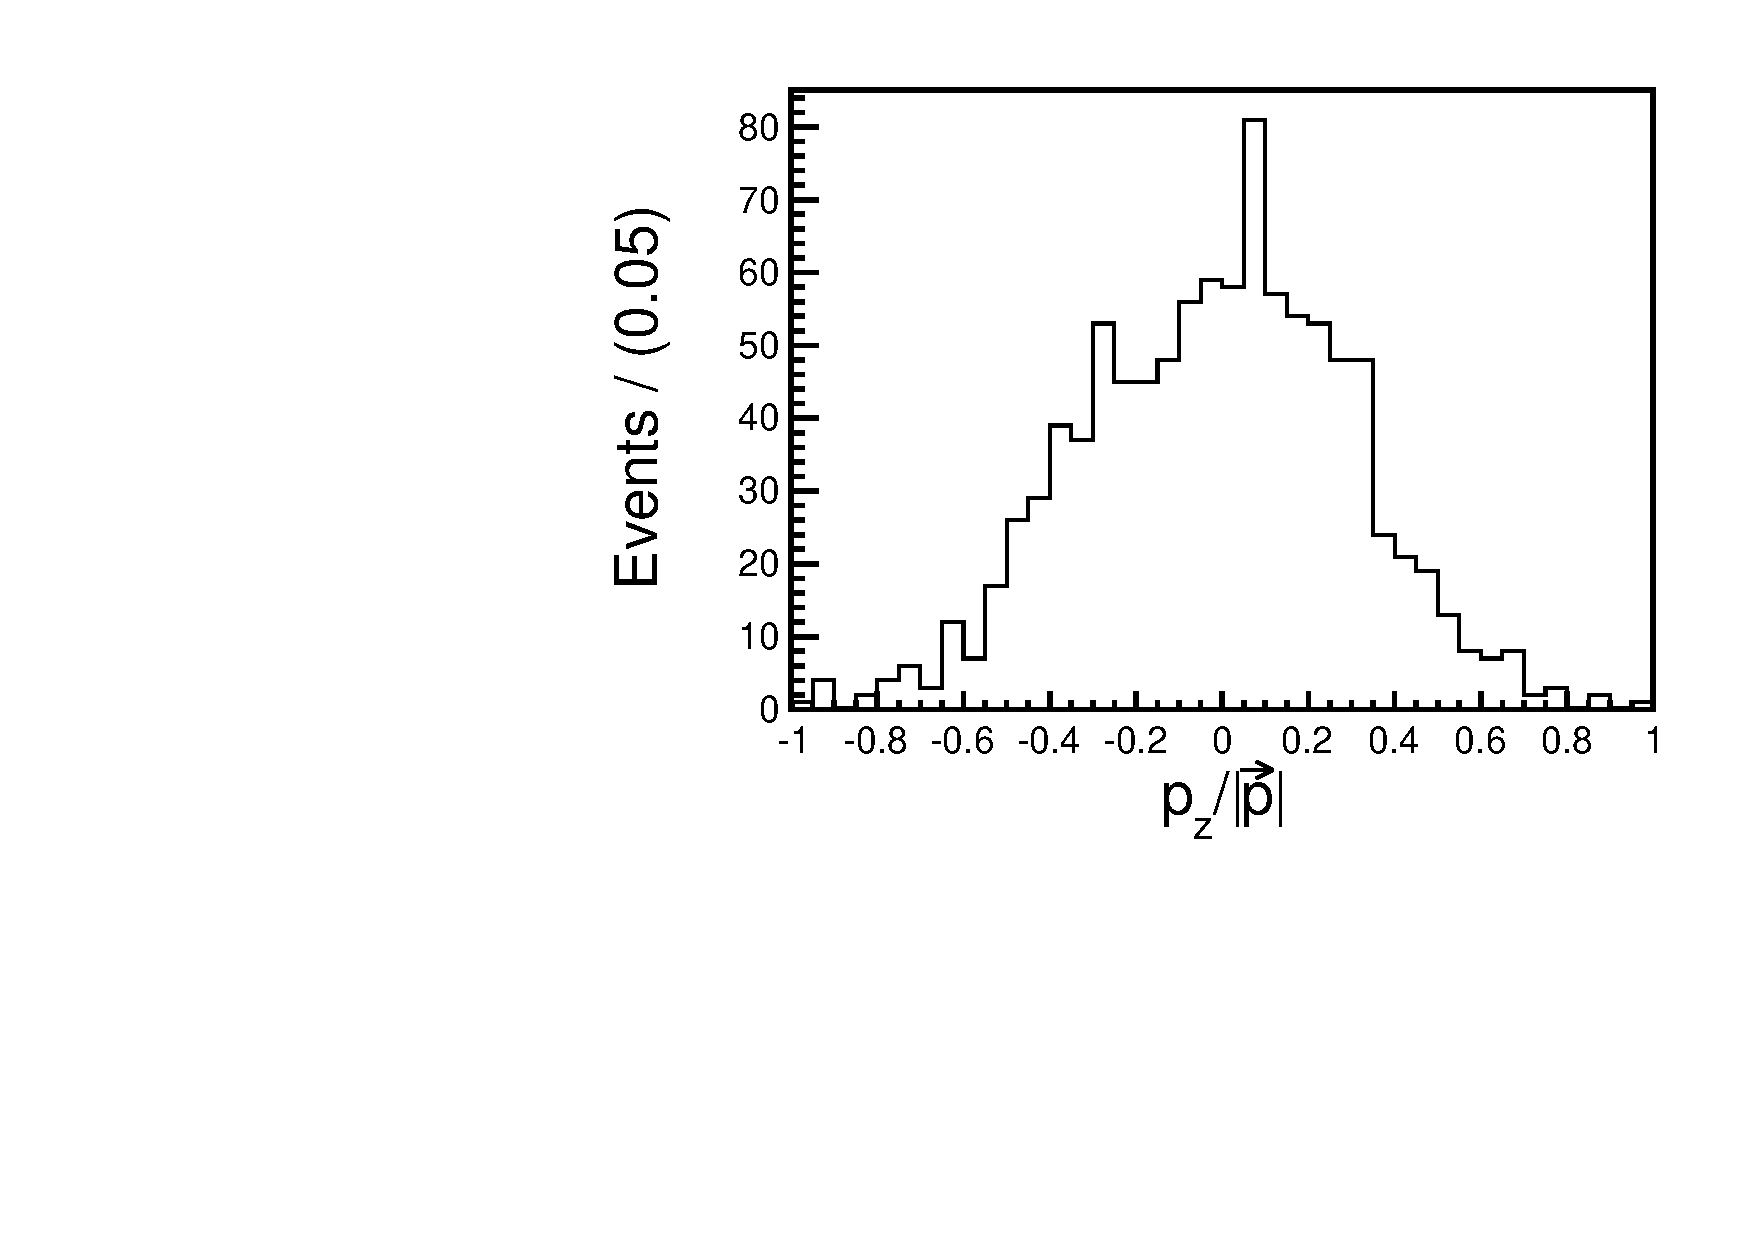
\includegraphics[scale=0.295]{graphs/hDirZ_v1.pdf}}
        %%\subfigure{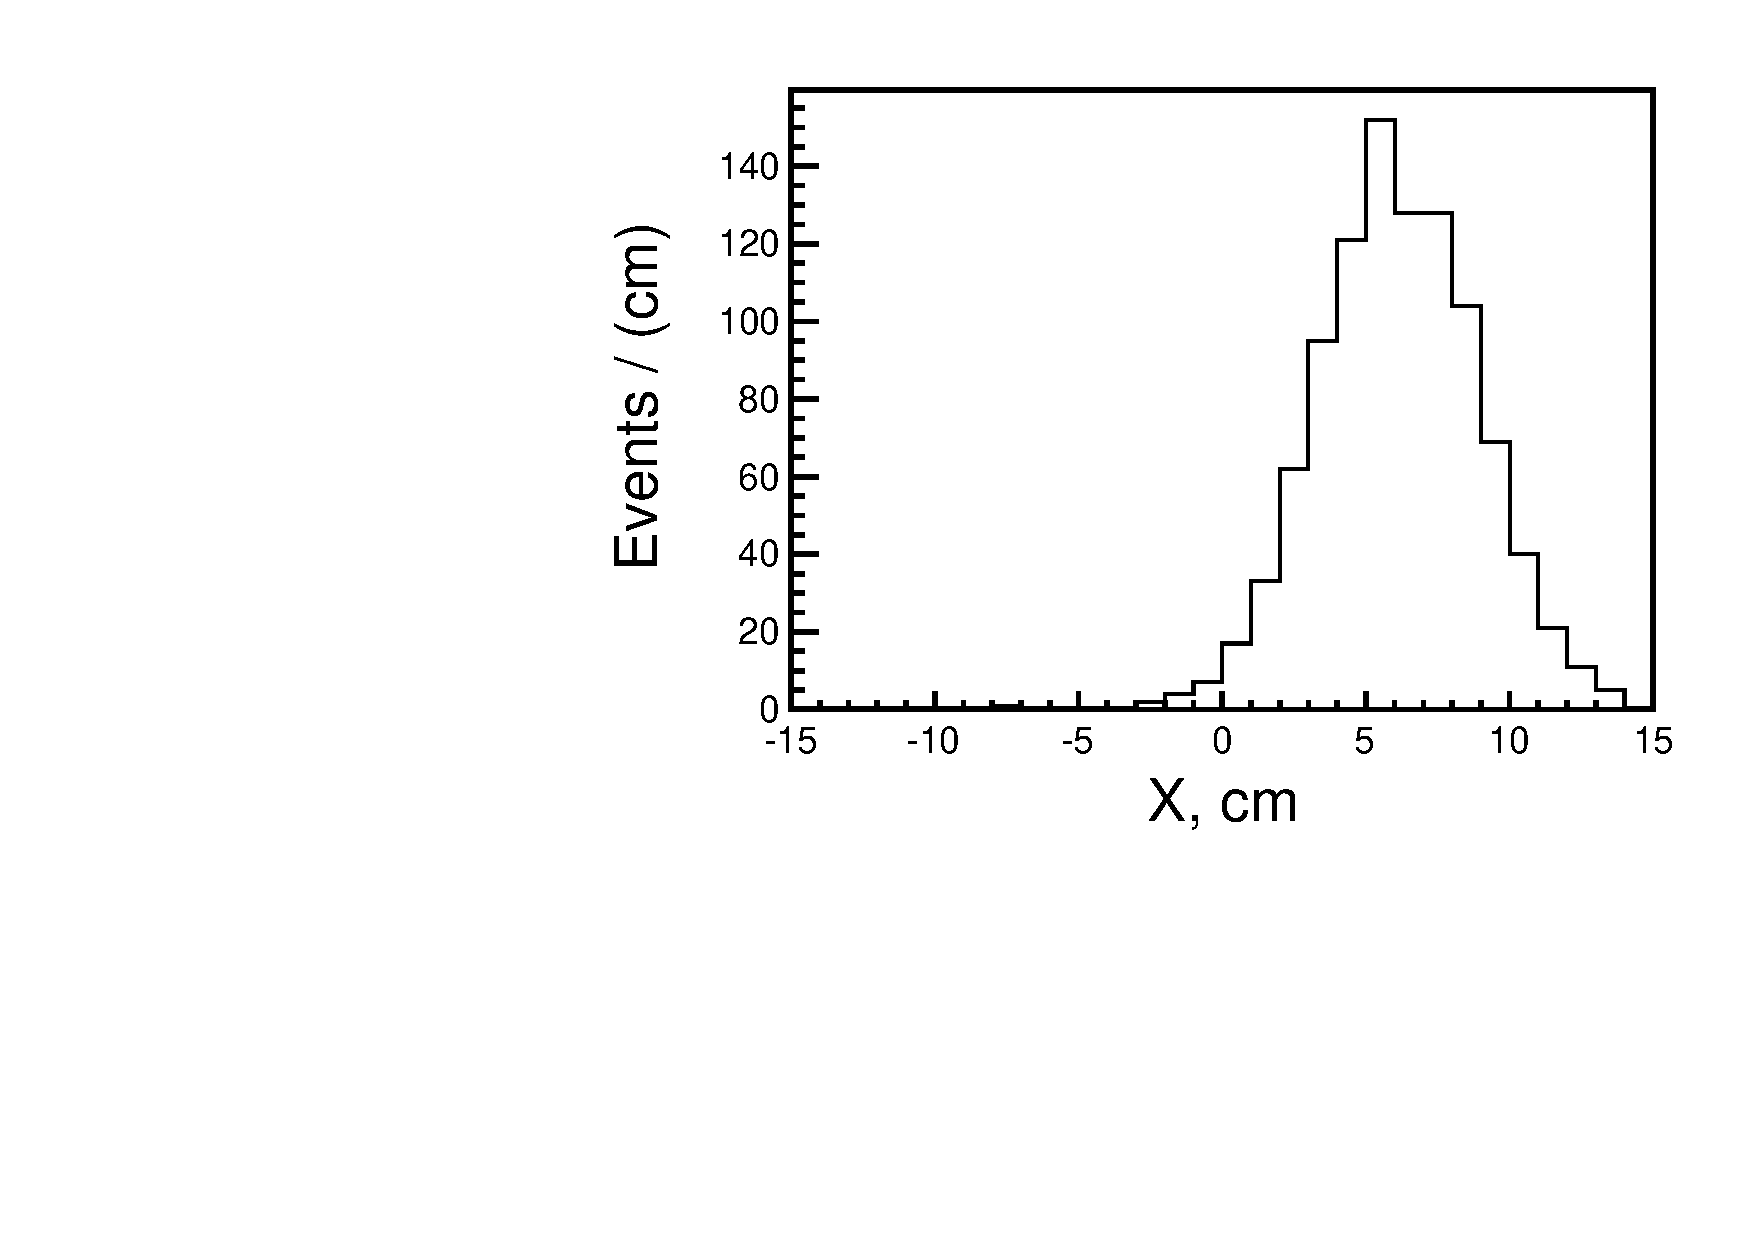
\includegraphics[scale=0.295]{graphs/hVtxX_v1.pdf}}
        %%\subfigure{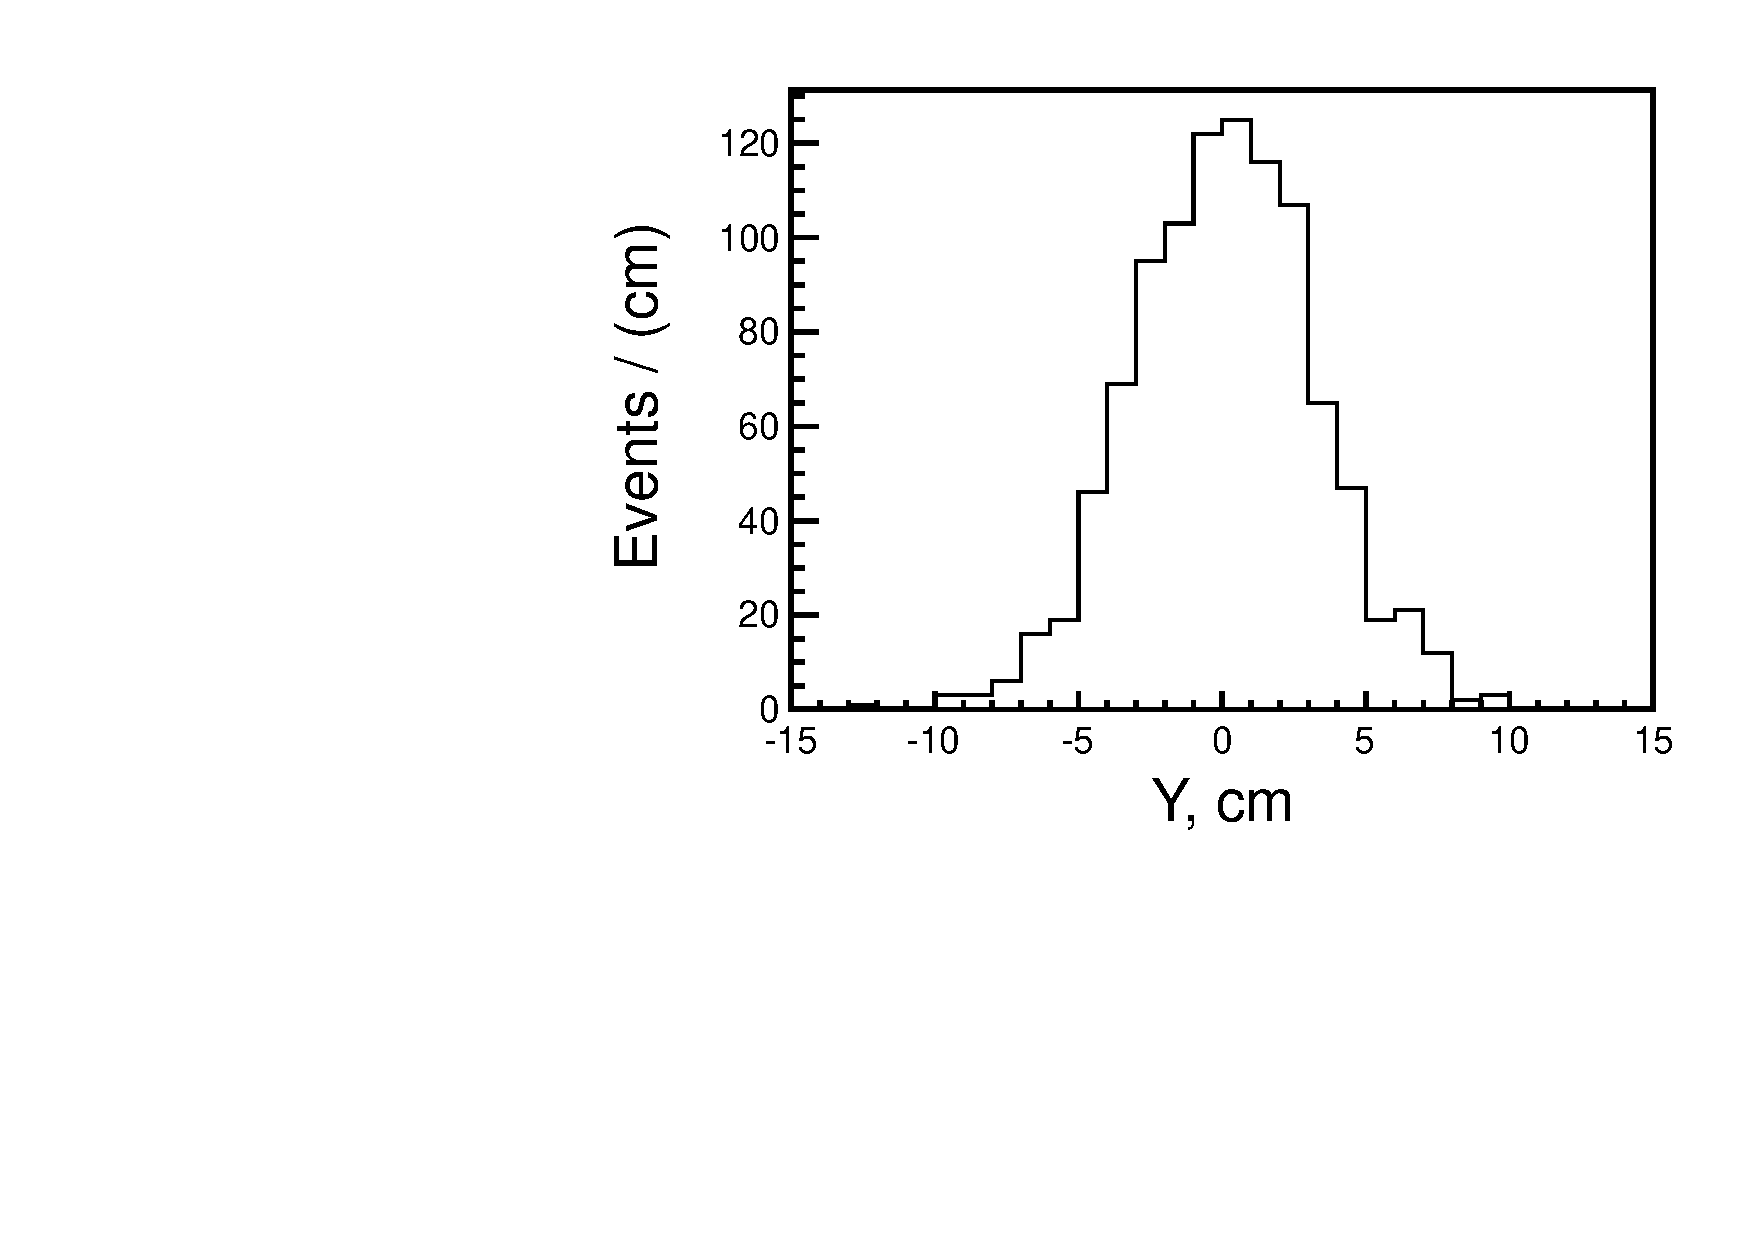
\includegraphics[scale=0.295]{graphs/hVtxY_v1.pdf}}
        %%\subfigure{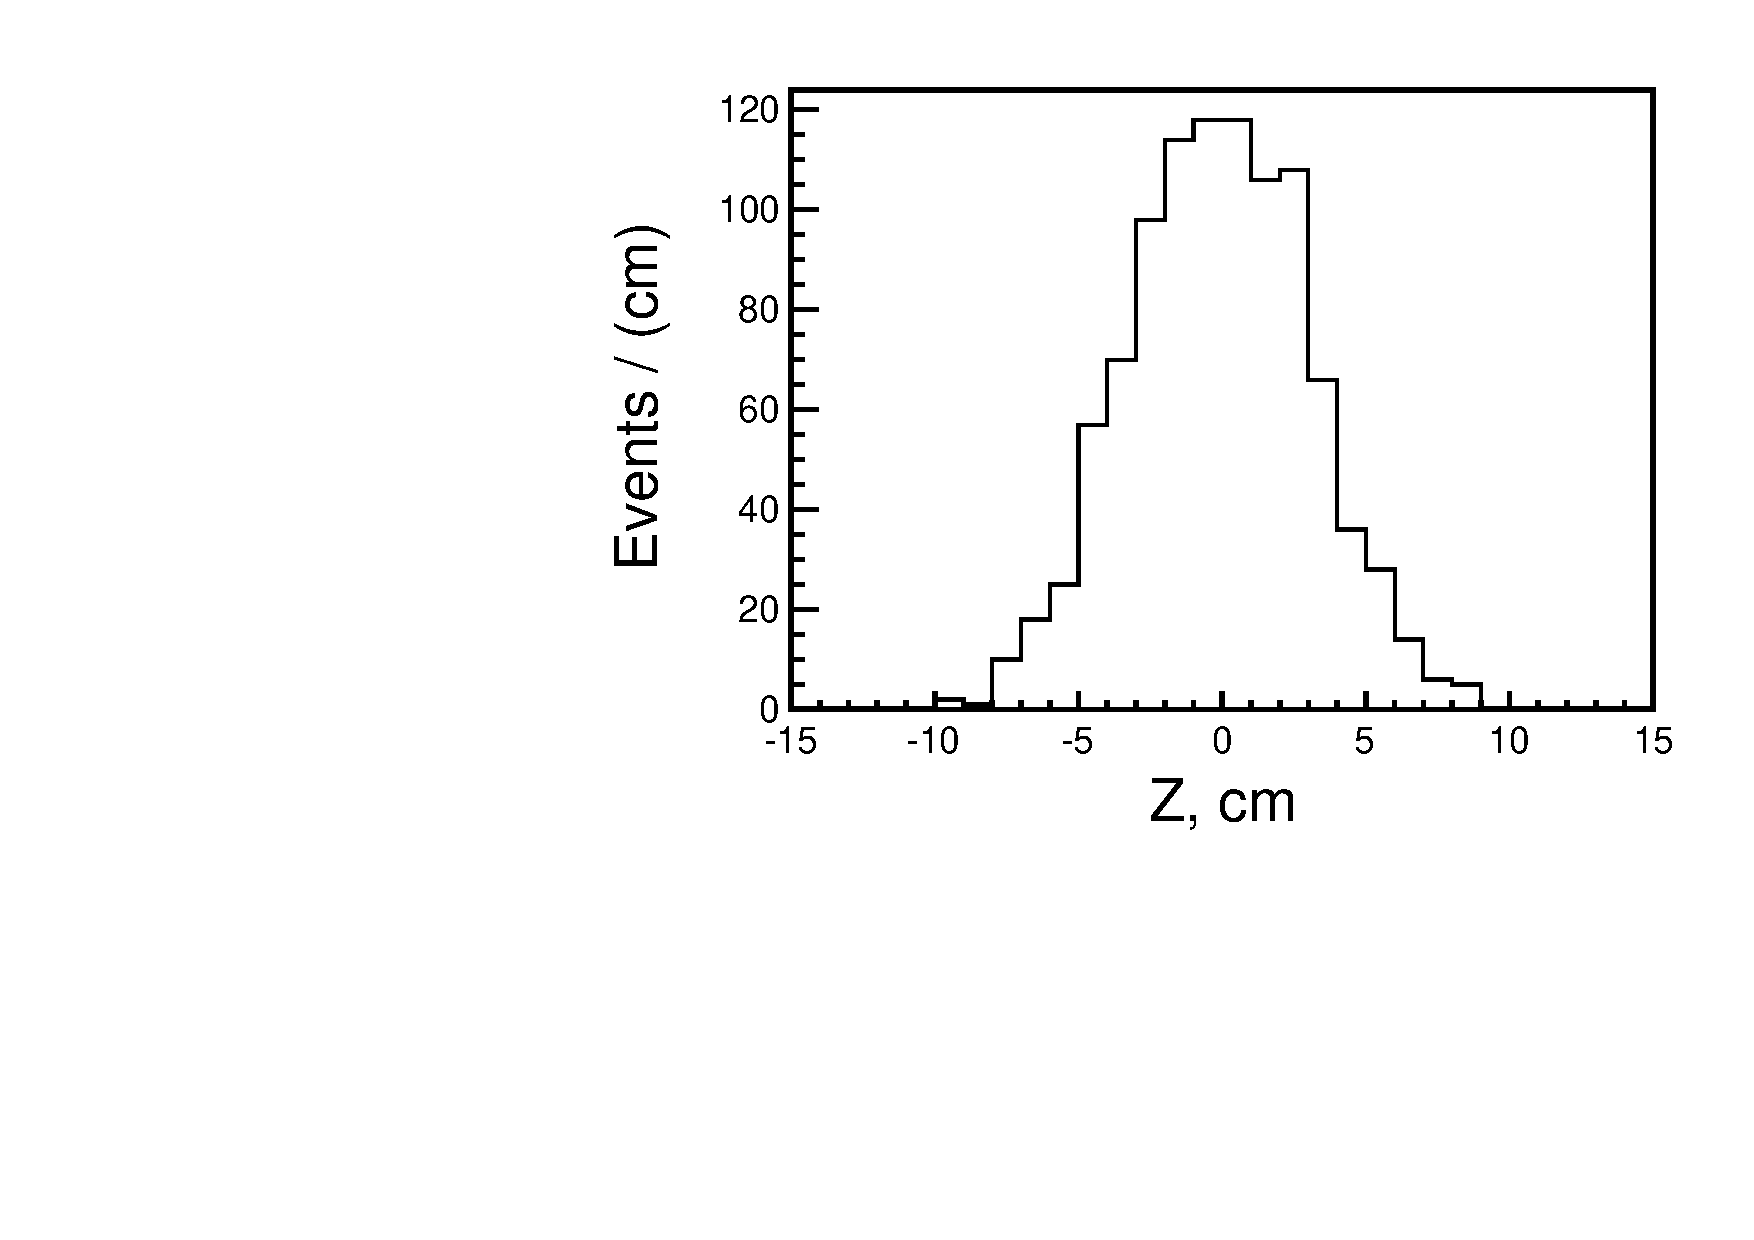
\includegraphics[scale=0.295]{graphs/hVtxZ_v1.pdf}}
        \subfigure{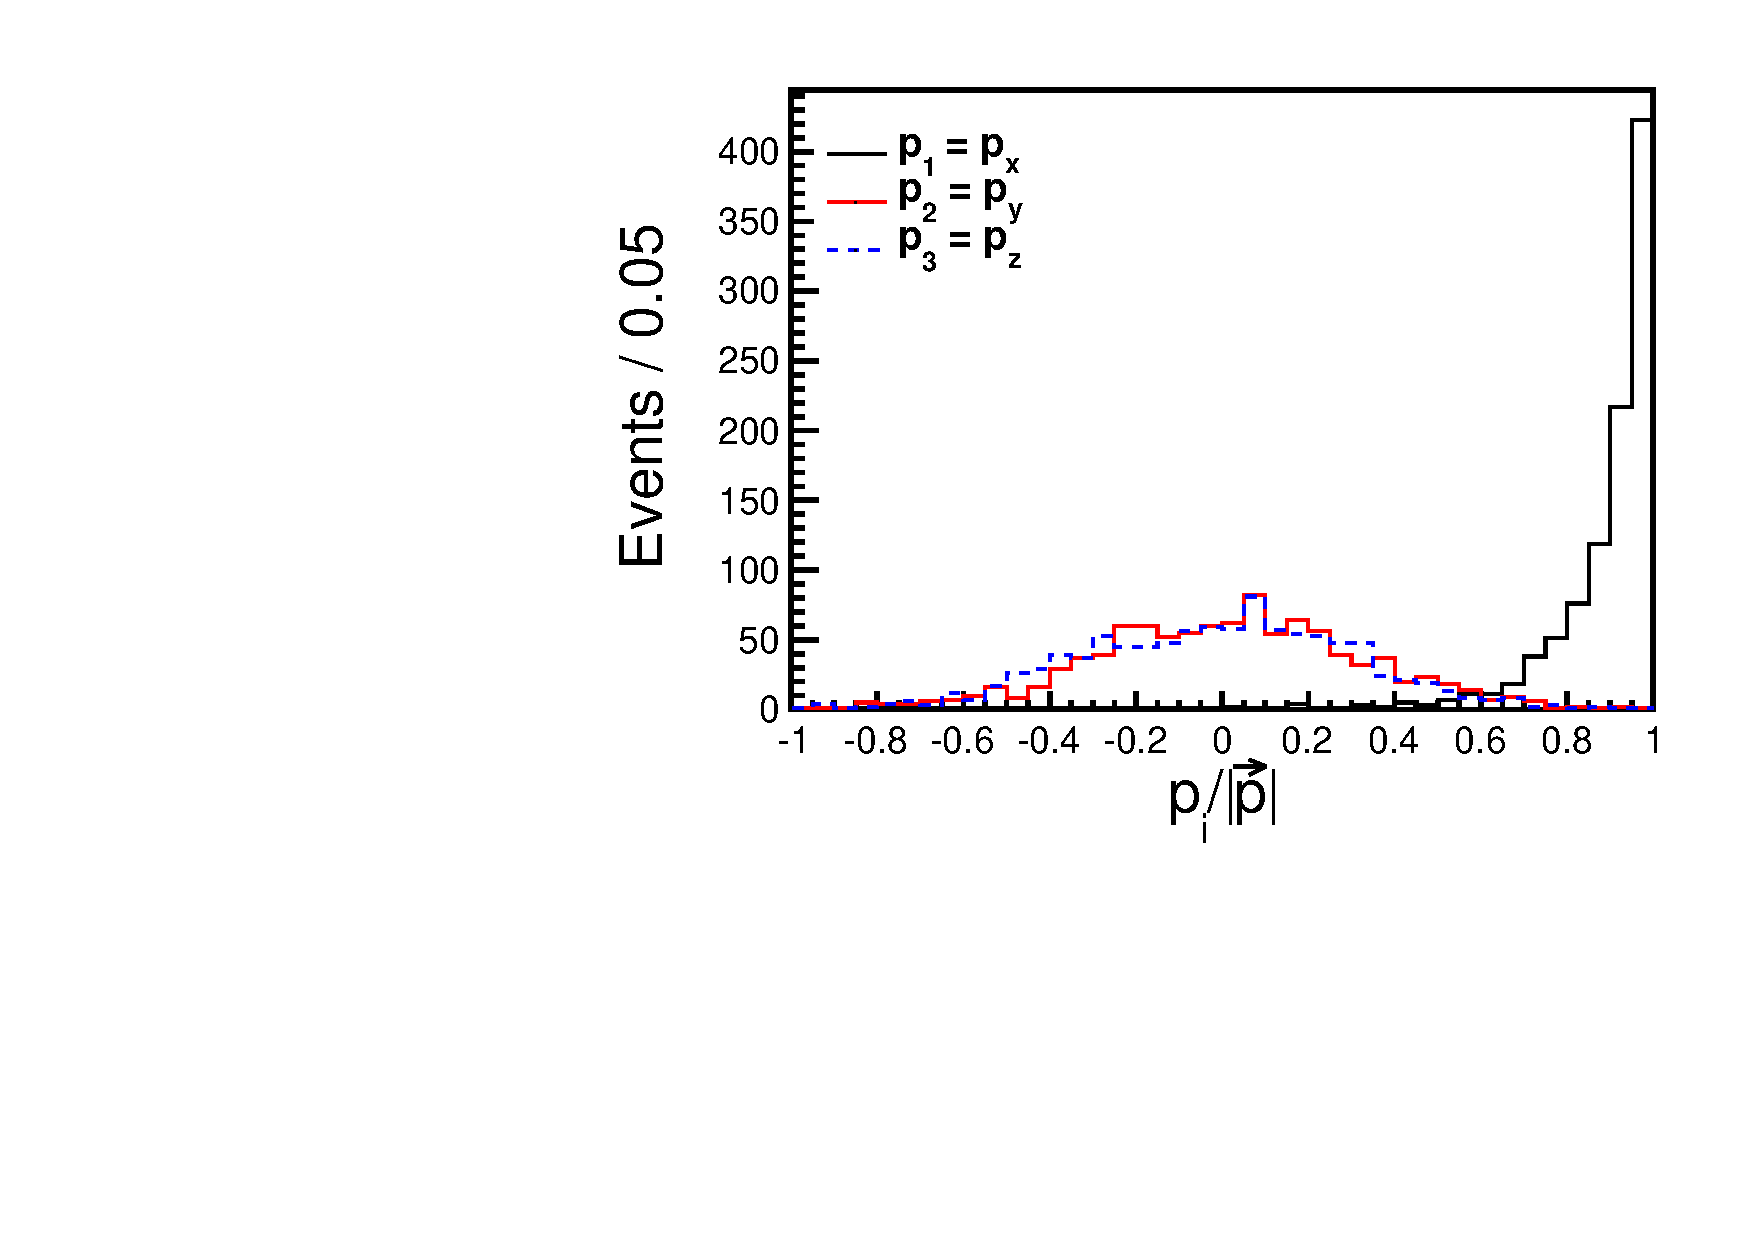
\includegraphics[scale=0.375]{graphs/hDir_34ns.pdf}}
        \subfigure{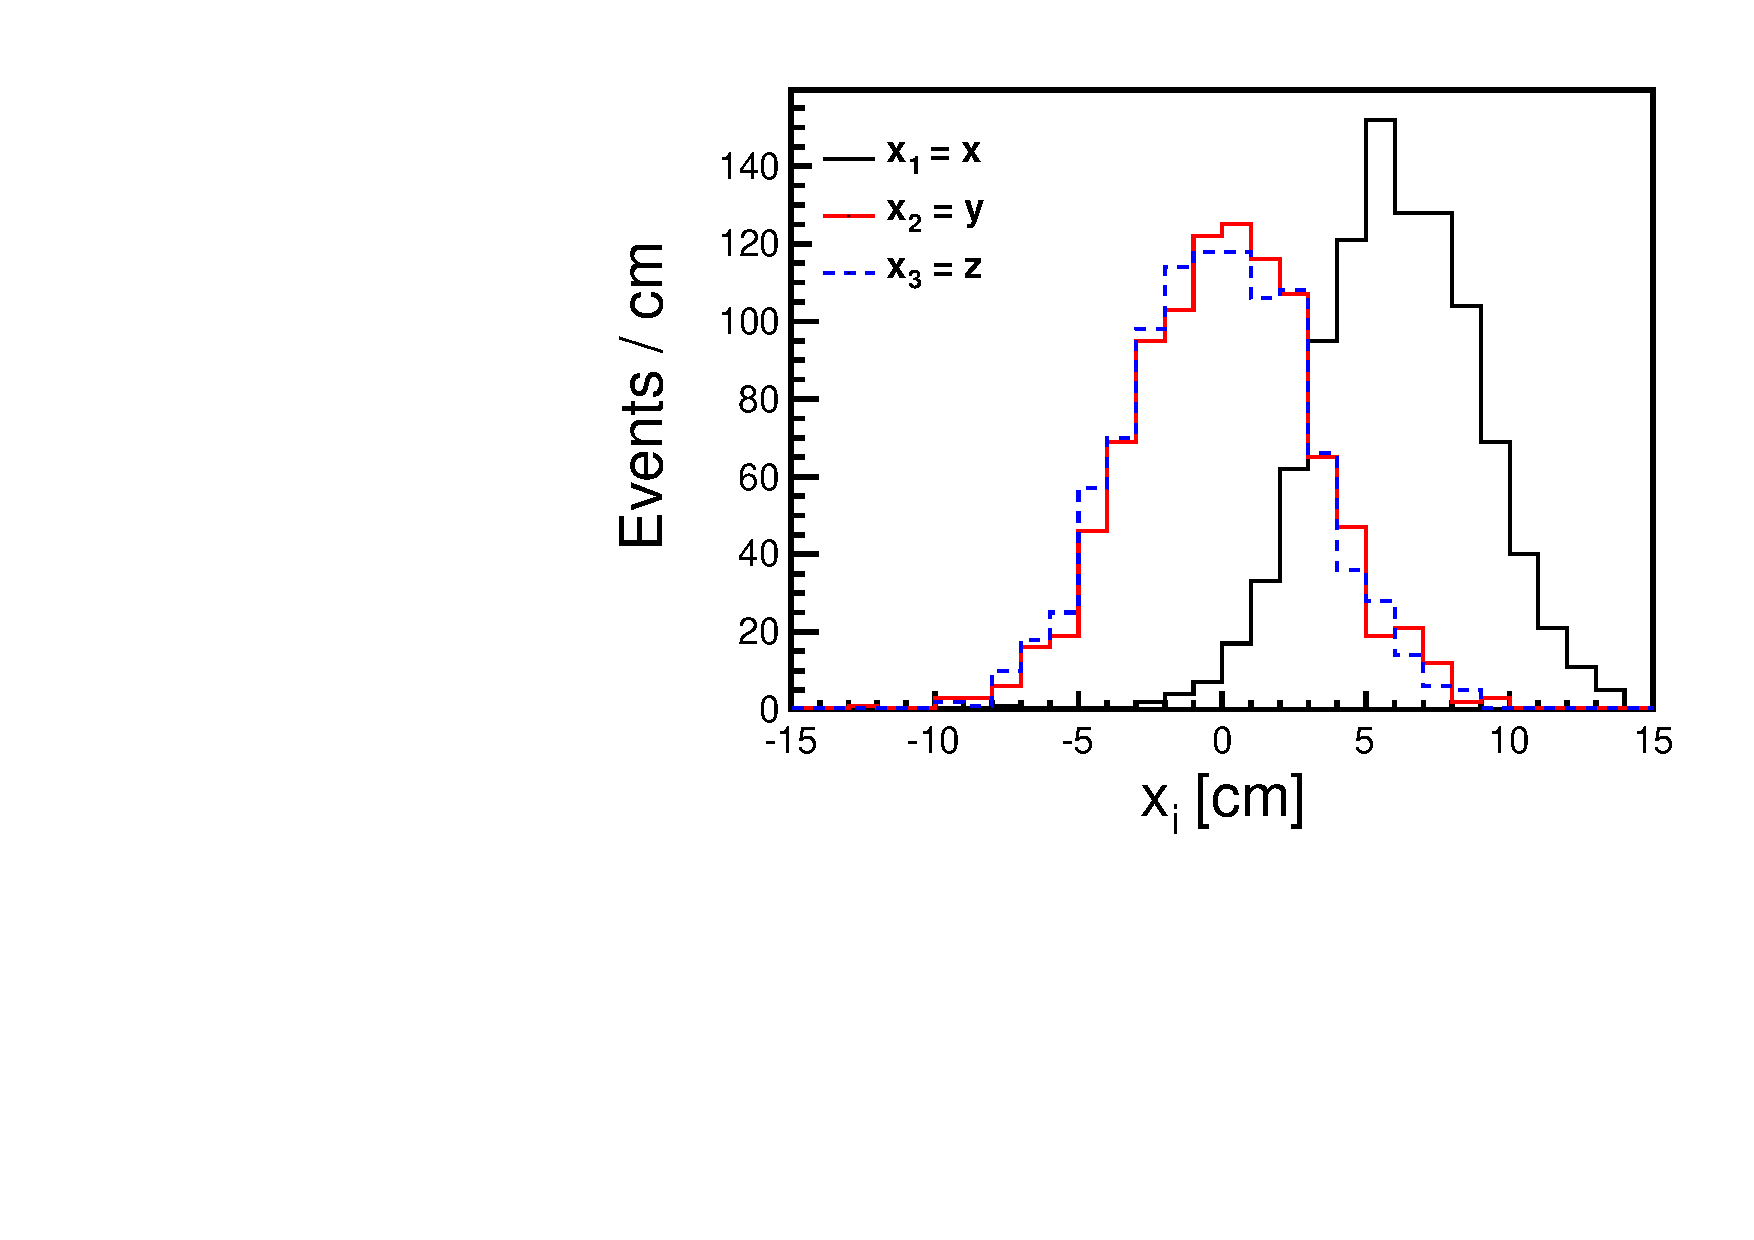
\includegraphics[scale=0.375]{graphs/hVtx_34ns.pdf}}
        \caption[]{\label{fig:reco} (Left) The reconstructed direction,
        $(p_x/|\vec{p}|, p_y/|\vec{p}|,
        p_z/|\vec{p}|)$, for the simulation of 1000 electrons
        (5~MeV). In the simulation the electrons are produced along the
        x-axis, $\vec{p}/|\vec{p}|$ = (1,0,0), and originate
        from the center of the 6.5m-radius detector, $\vec{r}$ =
        (0,0,0). Only photons with arrival time of $t<$ 34.0~ns are used
        in the reconstruction. The quantum efficiency of the bialkali
        photocathode is taken into account. (Right) The reconstructed
        vertex position, $(x,y,z)$, for the same simulation.}
\end{center}
\end{figure}

\section{Reconstruction}
\label{reconstruction_sec}

The timing studies show that in the early time window, $t\leq$
34.0~ns, the ratio $R_{C/S}$ is high, improving the photoelectron hit selection. In this section, we apply
reconstruction tools for a water Cherenkov detector, WCSimAnalysis,
to the problem of reconstructing the position and direction of 5~MeV
electrons from this early light.  WCSimAnalysis is a water Cherenkov
reconstruction package developed for the Long Baseline Neutrino
Experiment (LBNE collaboration)\cite{Blake}. It provides a framework
for generic event cleaning, track reconstruction, and particle
identification, and comes equipped with variety of pre-built
algorithms. It is continuing to be expanded using new track-fitting
techniques for water Cherenkov detectors\cite{Sanchez2012525} based on
advanced photosensors with sub-cm imaging capabilities and timing
resolutions below 100 picoseconds\cite{LAPPDSum,LAPPDTDR}.

The results presented in this paper rely on a simple vertex
reconstruction algorithm, commonly known as a ``point
fit''\cite{SuperKalgo}. It assumes that all of the scintillation and
Cherenkov light is emitted from a single point in space-time
$(x_0,y_0,z_0,t_0)$. In actuality, the light is emitted along an
extended, multi-scattered electron track. However, at the energies
discussed in this paper, the extent of this track is small (a few cm)
compared to the scale of the detector (R=6.5 meters) and therefore the typical
photon transit distances.

The first step of the reconstruction process relies on exact numerical
calculations of vertex candidates from quadruplets of hits. Given a
single point source, we need four constraints to solve for the four
unknowns of the vertex $(x,y,z,t_0)$\cite{Smy}. This approach
would provide an exact solution in the case of four prompt,
un-scattered photons originating from a common point. However, many of
these randomly chosen quadruplets will produce anomalous solutions due
to `real world' effects such as delayed emission and deviations from the
point-like geometry. Nonetheless, we found that any chosen subset of
400 quadruplets was a sufficiently large ensemble to assure that some
solutions will be close to the true vertex.

Once a set of vertex candidates has been found, we test the goodness
of each vertex and select the one that best fits the full ensemble of
photon hits. The goodness of fit is determined based on the
distribution of an observable known as the ``point time
residual''\cite{SuperKalgo}. The point time residual is calculated by
taking the difference between the measured time of a photon hit, and
the predicted time of the hit, given its distance from the vertex
hypothesis, a single effective speed of light in the scintillator, and
the hypothesized $t_0$ of the event. The width of the time residual
distribution over all hits is minimized when the hypothesized vertex
is near the true vertex. Based on this figure of merit, we select the
vertex with the narrowest time residual distribution from among the
400 candidates.

The direction of the electron track is then determined by taking the
centroid of all vectors pointing from the fitted vertex to the hits on
the detector. Since the Cherenkov light is highly directional, and
since the timing cut enhances the purity of the Cherenkov light in the
sample, this calculation provides a good measure of the track
direction. 

For the purpose of testing the reconstruction algorithm we use 1000
simulated electrons with an energy of 5~MeV, lower energies are studied in the next section.
The electrons are simulated at the center of the detector, $\vec{r}$ = (0,0,0), along
the x-axis, $\vec{p}/|\vec{p}|$ = (1,0,0). Figure \ref{fig:reco}
shows the vertex reconstruction. The vertex is reasonably well
reconstructed around the center of the detector, $\vec{r}$ = (0,0,0),
except along the x-axis. The RMS values of the distributions for all three
reconstructed coordinates are smaller than 3.5~cm. The shift along
the x-axis is due to two effects for which the reconstruction has to
use average values rather than the unknown true value for each
hit: the wavelength and hence the speed of the light in the medium,
and the point of emission for each of the photons, reconstructed
as coming from a common point. The reconstruction of the direction
also is shown in figure \ref{fig:reco}. It shows that for the majority
of the events the initial electron direction is reconstructed well.
This is a promising result given the simplicity of the algorithms
used.

\section{Energy dependence}
\label{edep_section}
In the previous sections we presented results on single 5~MeV electrons.
In this section we study two lower energies, 1.4~MeV and 2.1~MeV. These
energies correspond to Q/2 for the double beta decay of
$^{116}$Cd and $^{48}$Ca, respectively\cite{cd1,biller}. The isotope
$^{116}$Cd was chosen because of its potential use in quantum-dot-doped
scintillators\cite{qdot,qdot2} and $^{48}$Ca was chosen
to cover the Q-value range of $0\nu\beta\beta$ candidate isotopes.

\begin{figure}
        \begin{center}
        \includegraphics[scale=0.5]{graphs/PEandR_vs_energy_line.pdf}
        \caption[]{The energy dependence of the mean number of PEs after the 34.0~ns time cut is shown for Cherenkov-induced PEs (black circles) and scintillation-induced PEs (black squares). The ratio between the mean number of Cherenkov-induced and scintillation-induced PEs is shown as blue triangles connected by a line, values are given on the right y-axis. The statistical errors are too small to be seen. \label{Edep_NPE}}
        \end{center}
\end{figure}

The two additional simulation sets with 1.4 MeV and 2.1 MeV electrons were
generated using the default simulation configuration described in section
\ref{sim_section}. The PE time distribution for the default settings is shown
in figure \ref{time_plots_comparison} (a) for 5~MeV electrons. The shape
of the scintillation and Cherenkov spectra is similar for the lower energies (not
shown here). In figure \ref{Edep_NPE}, the energy-dependent mean number of
PEs per event after the 34.0~ns time cut is shown for Cherenkov-induced and
scintillation-induced PEs, as well as their ratio $R_{C/S}$. The mean number
of PEs from Cherenkov (scintillation) light is 21.8 (52.1), 38.4 (76.8)
and 108 (171) for 1.4~MeV, 2.1~MeV and 5~MeV, respectively. This gives the
ratios $R_{C/S}$ = 0.42, 0.50 and 0.63: The decrease in Cherenkov-induced
PEs is stronger than the decrease in scintillation-induced PEs as the energy
is lowered.

\begin{figure}[tbh]
        \begin{center}
        %%\subfigure{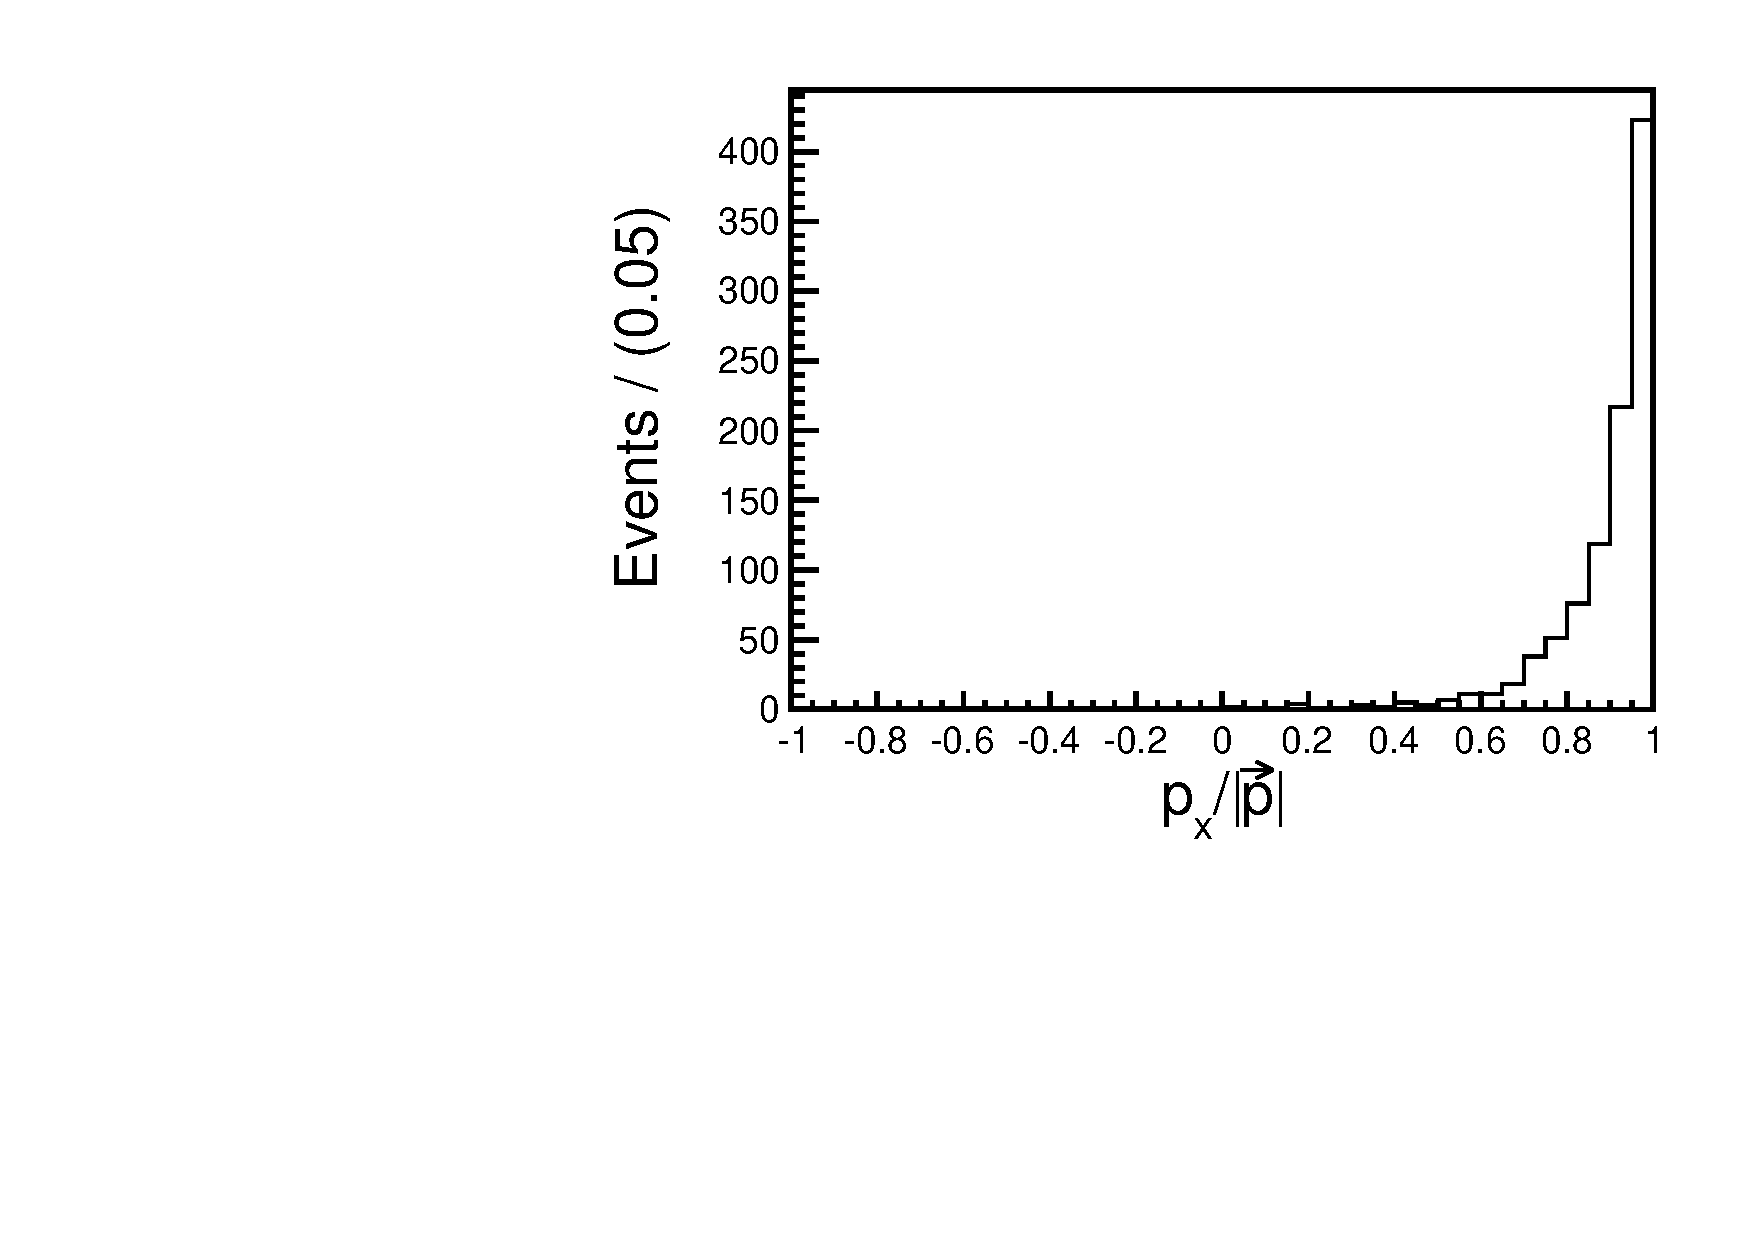
\includegraphics[scale=0.295]{graphs/hDirX_v1.pdf}}
        %%\subfigure{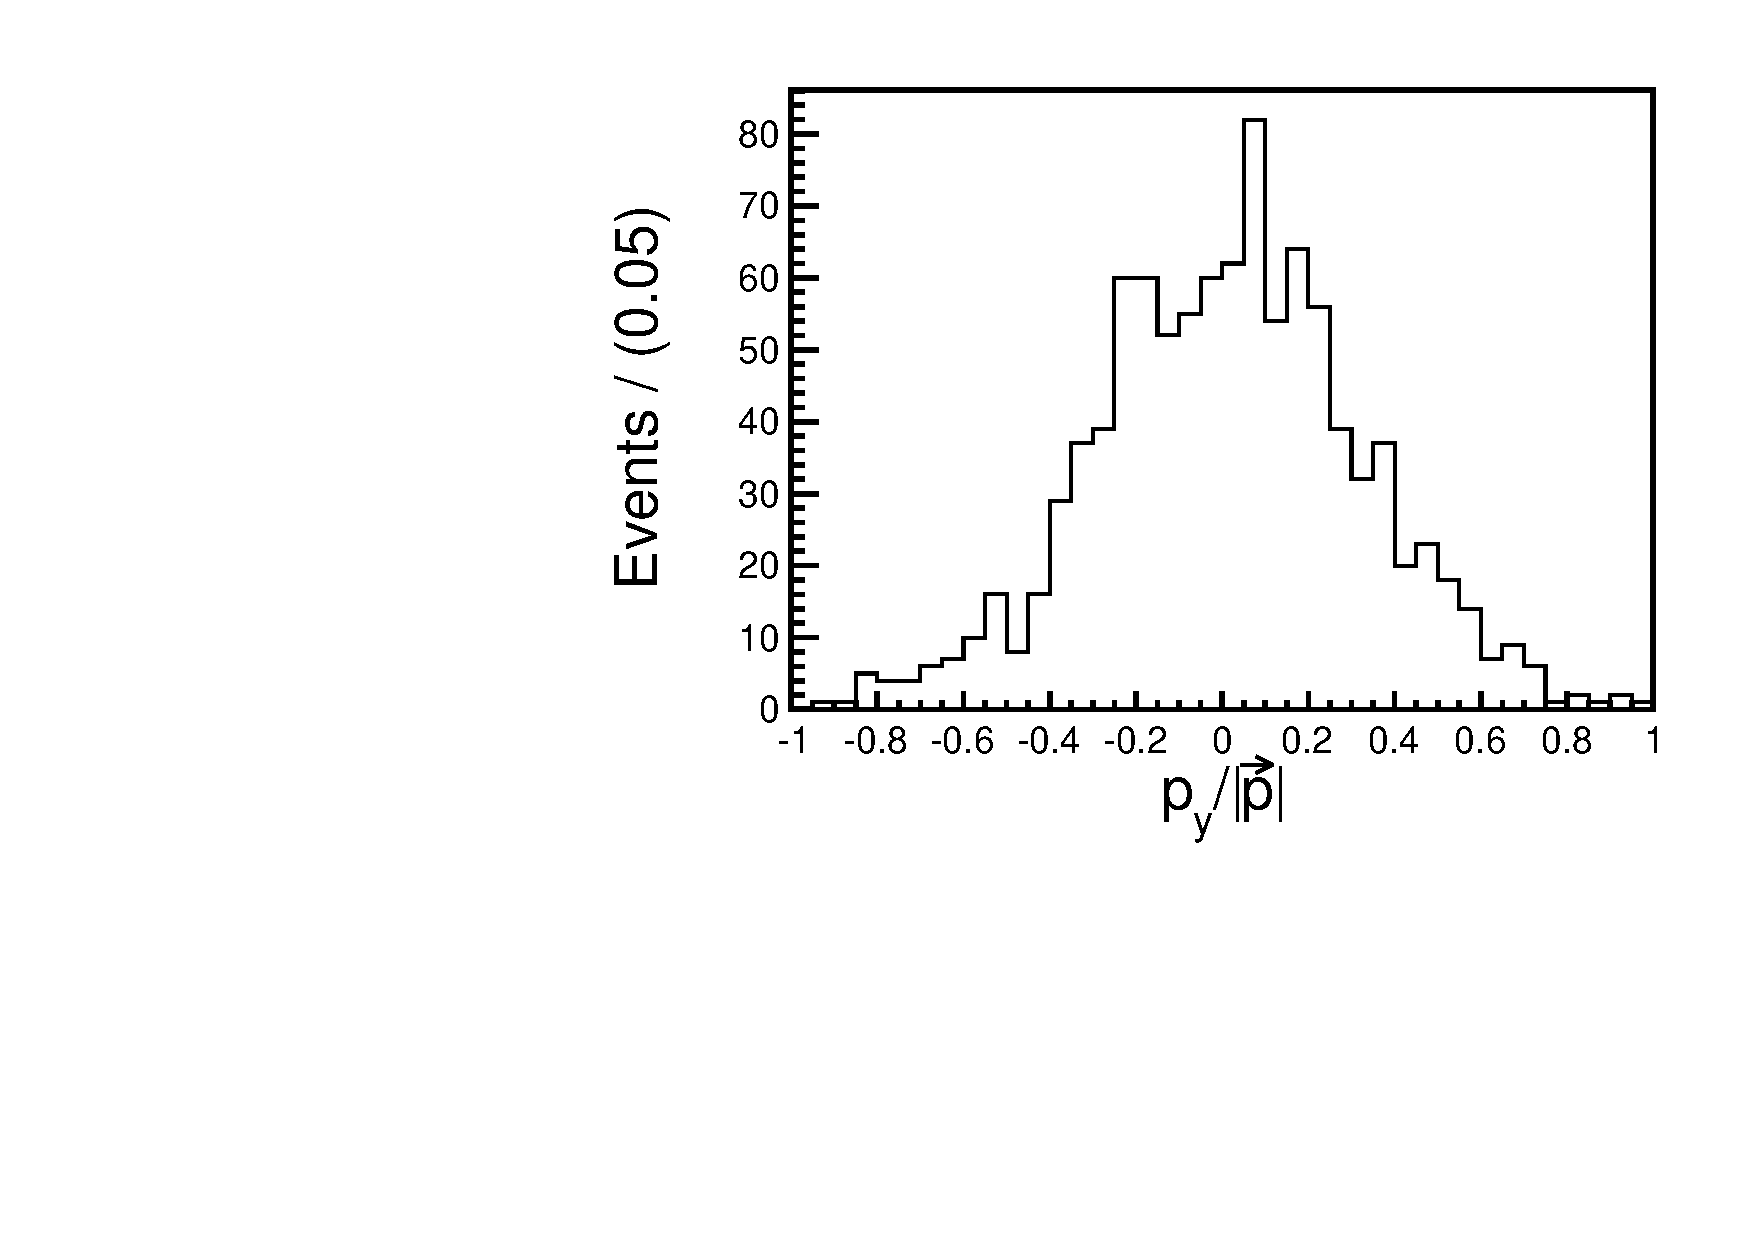
\includegraphics[scale=0.295]{graphs/hDirY_v1.pdf}}
        %%\subfigure{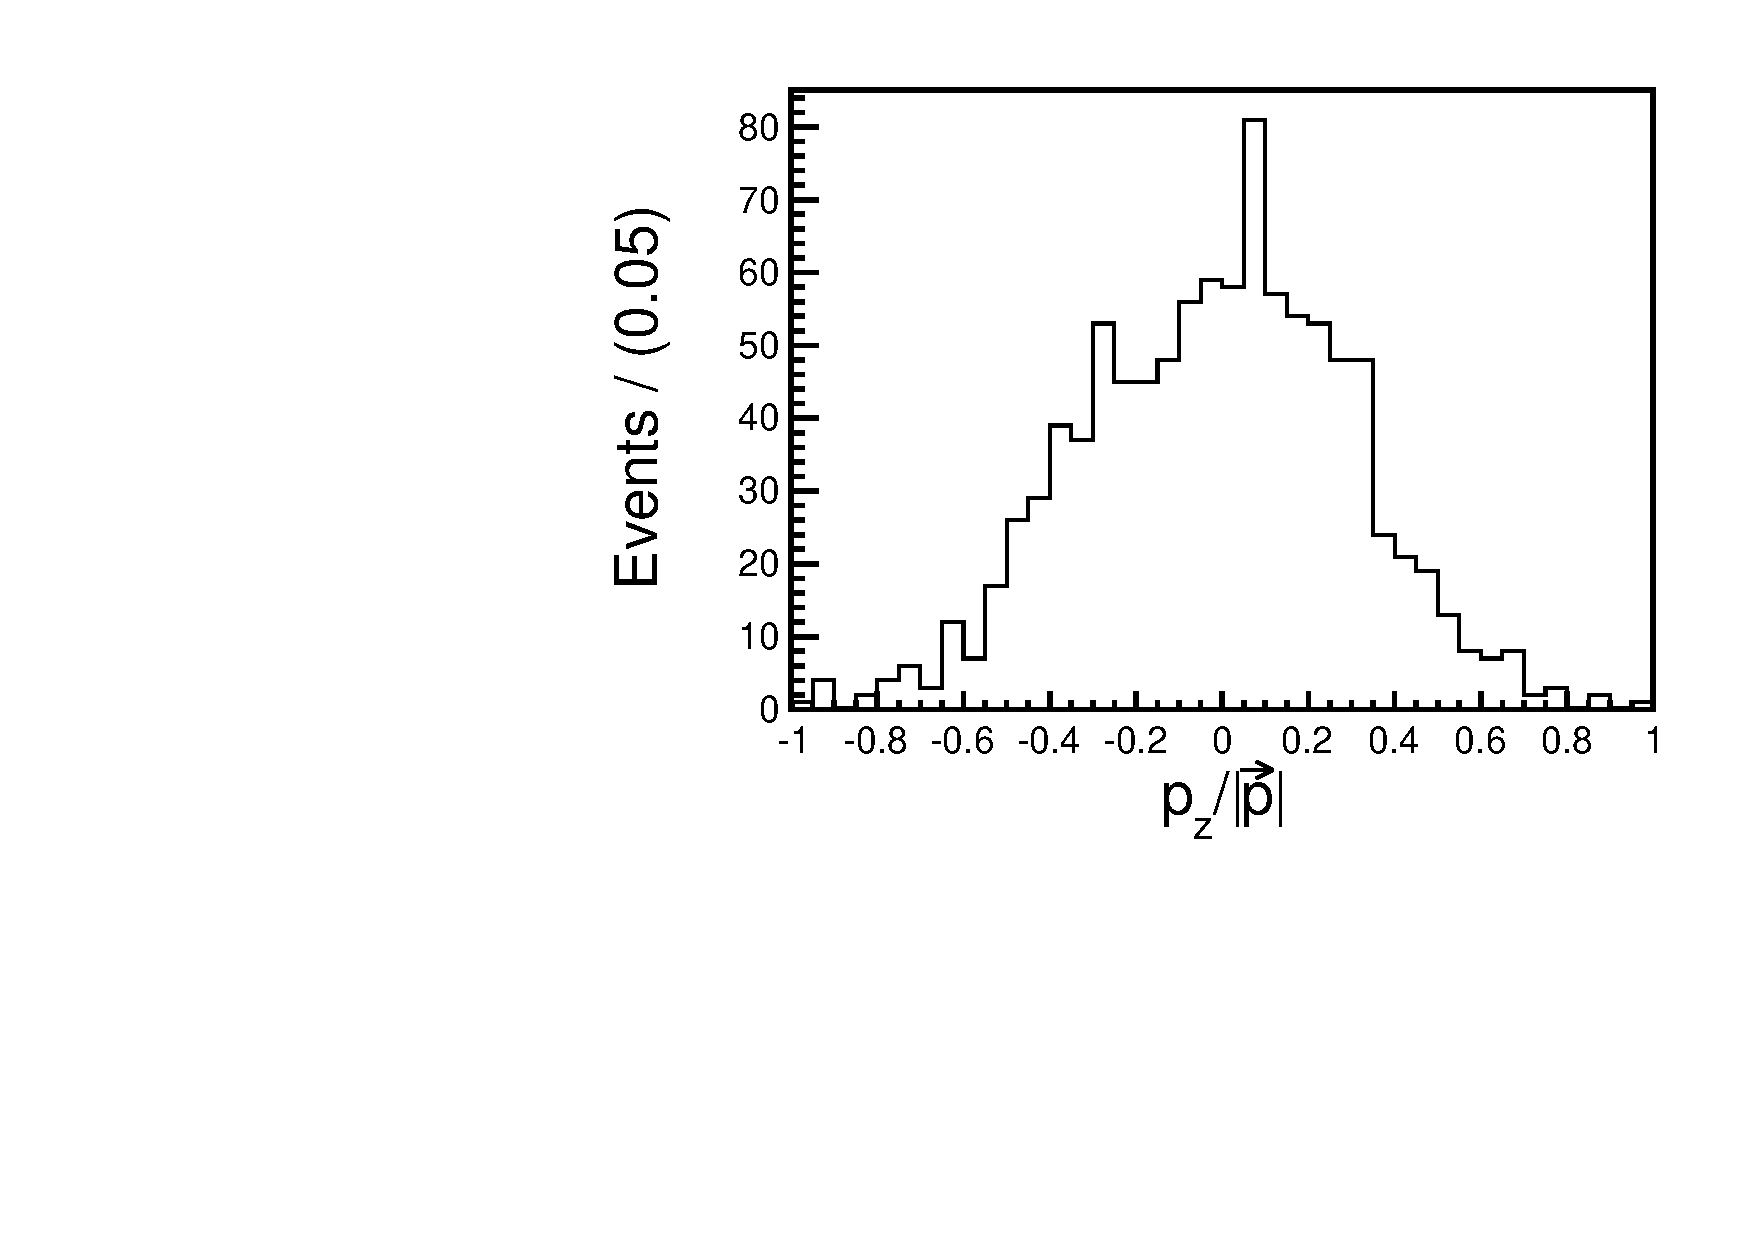
\includegraphics[scale=0.295]{graphs/hDirZ_v1.pdf}}
        %%\subfigure{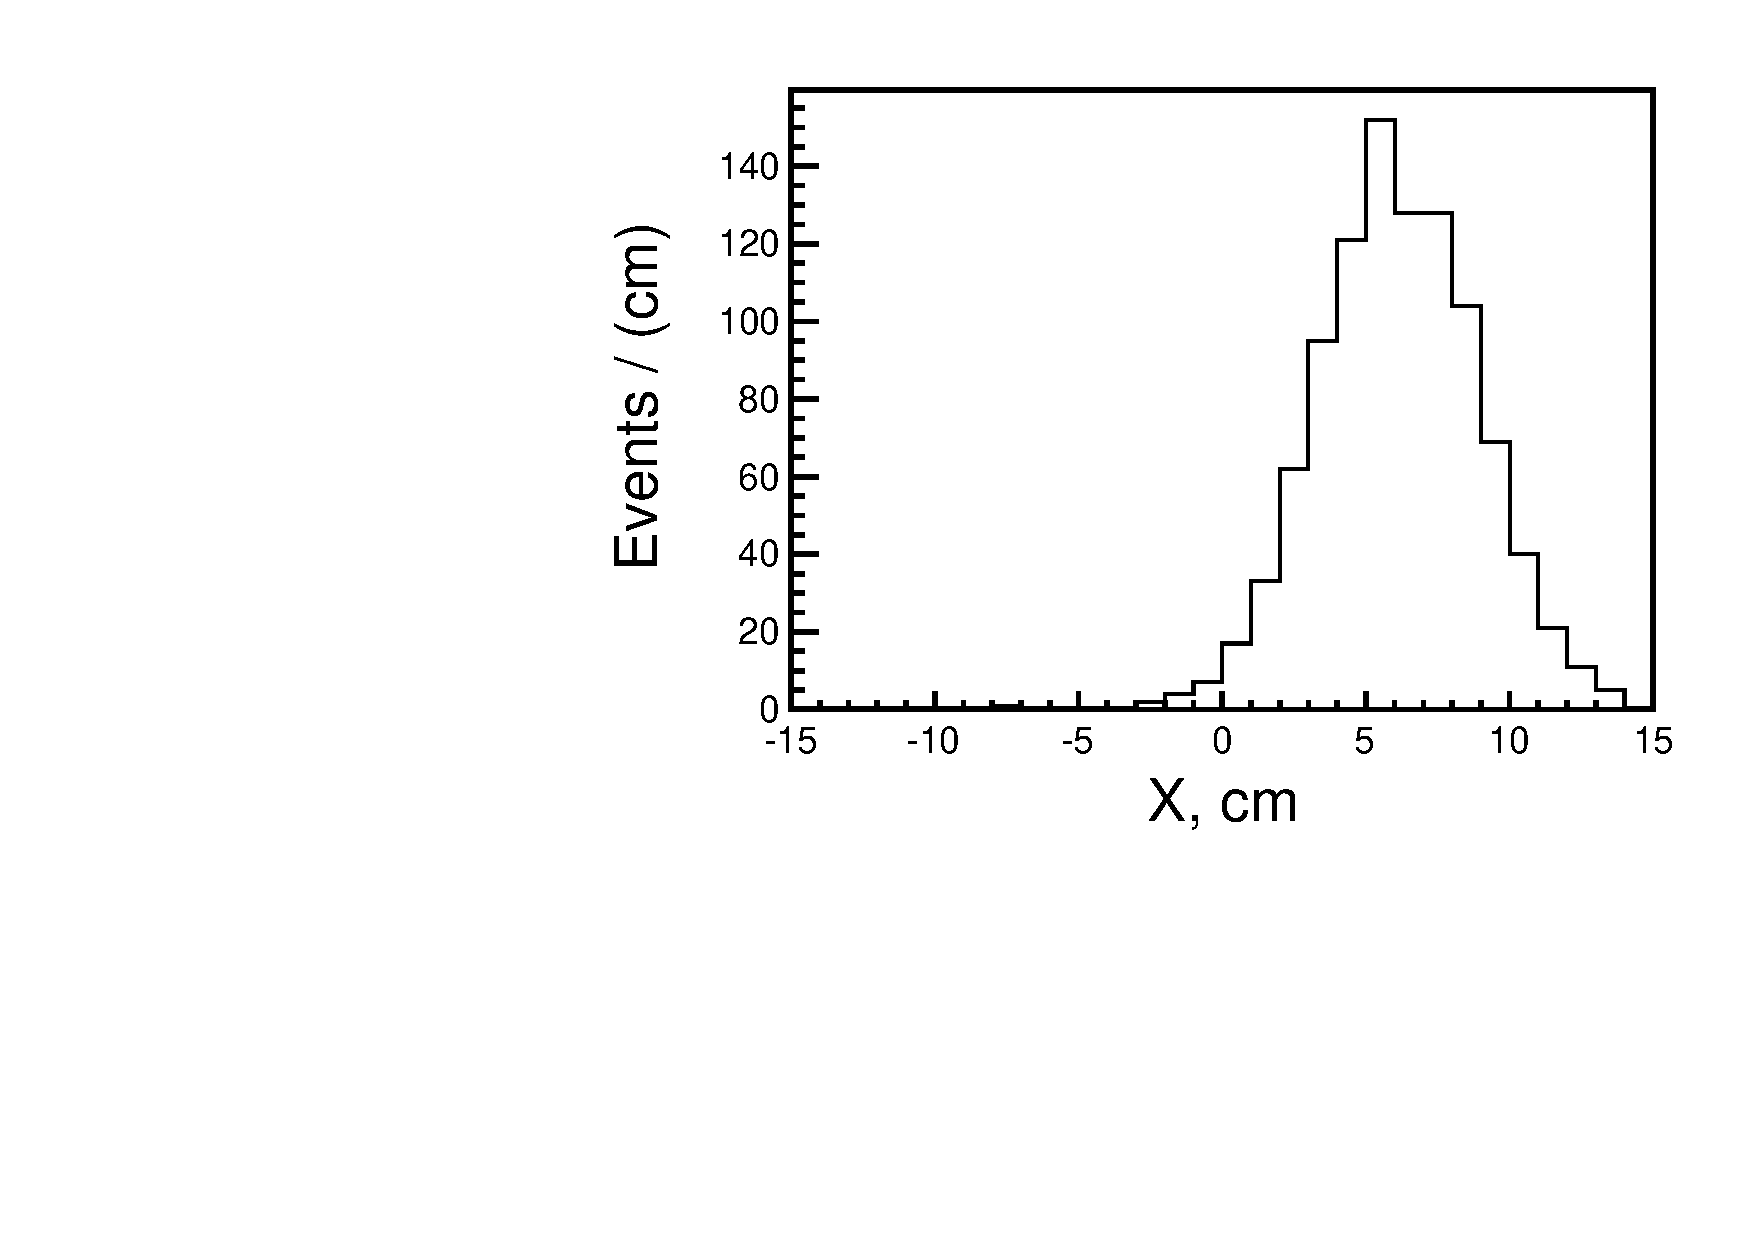
\includegraphics[scale=0.295]{graphs/hVtxX_v1.pdf}}
        %%\subfigure{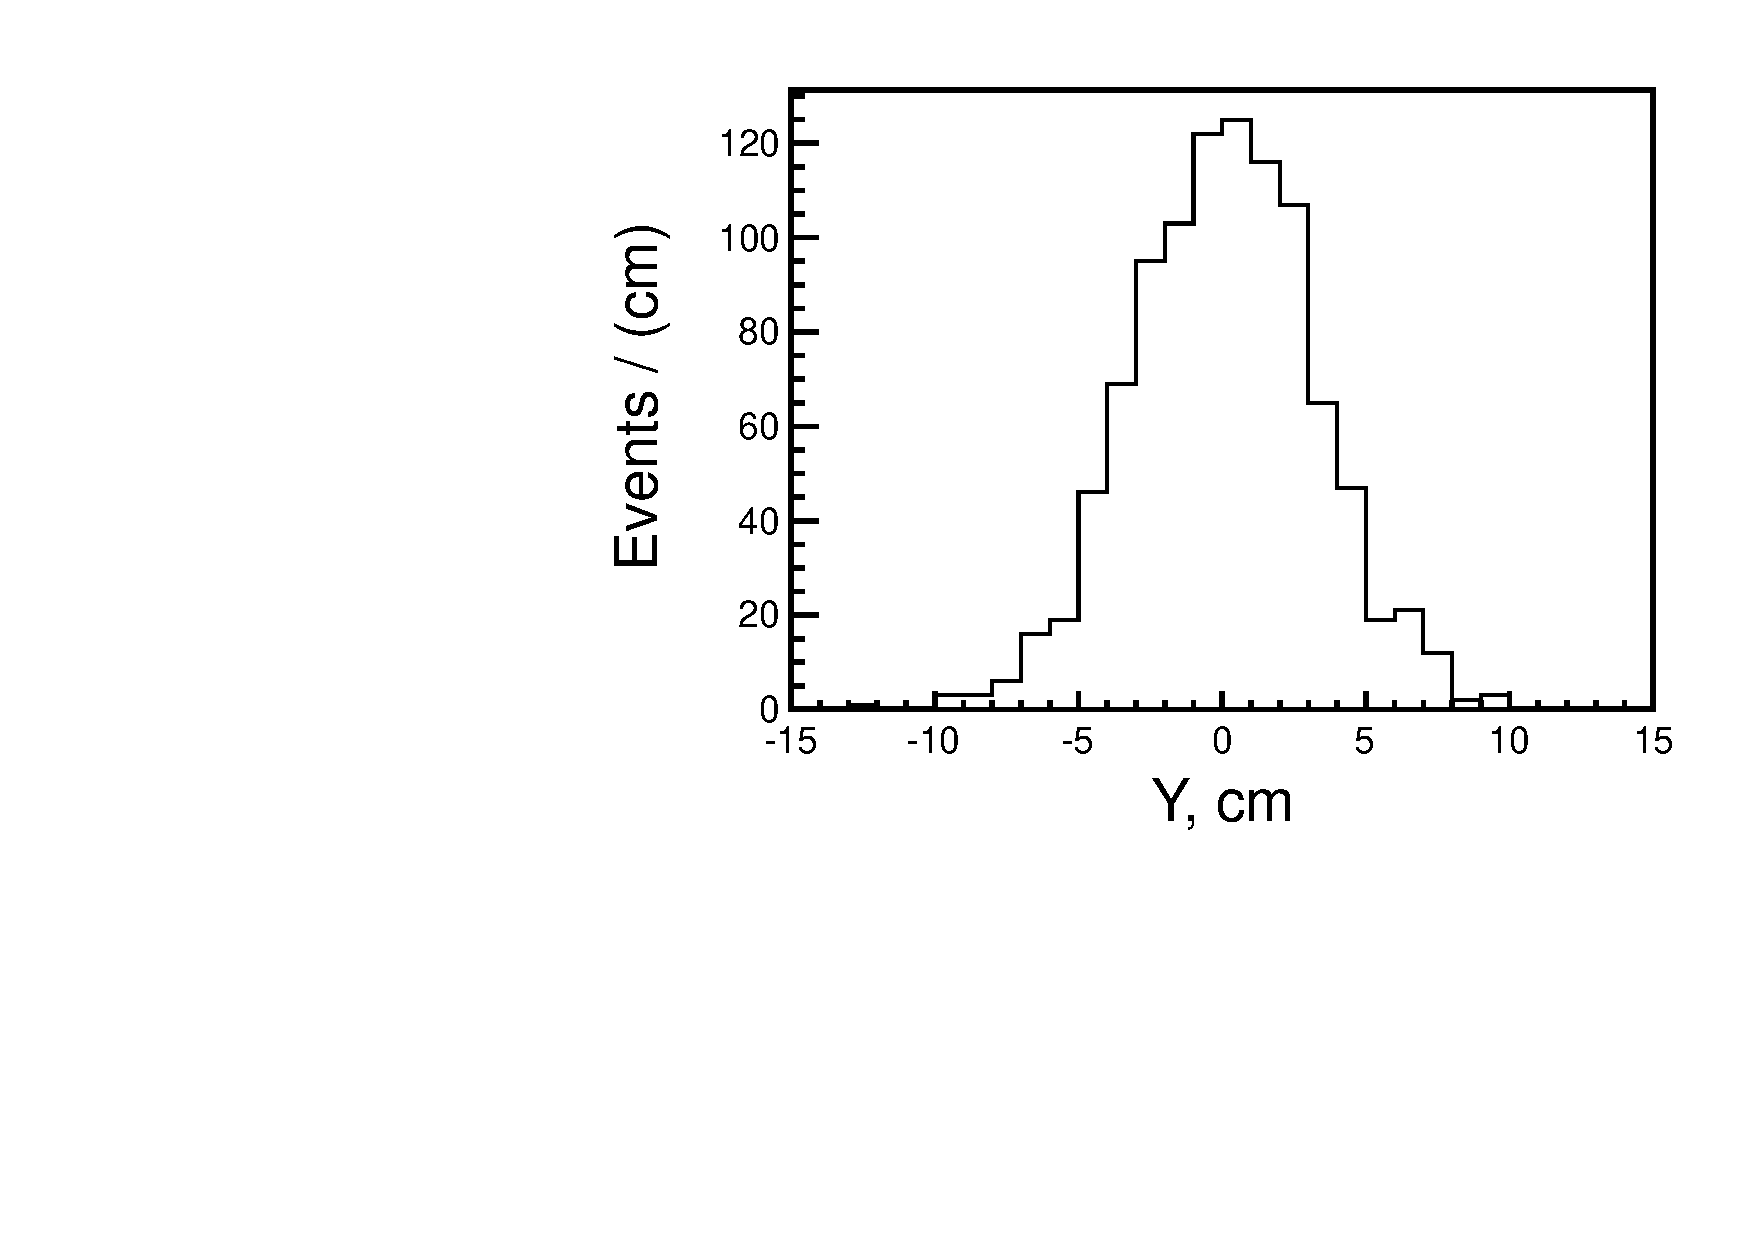
\includegraphics[scale=0.295]{graphs/hVtxY_v1.pdf}}
        %%\subfigure{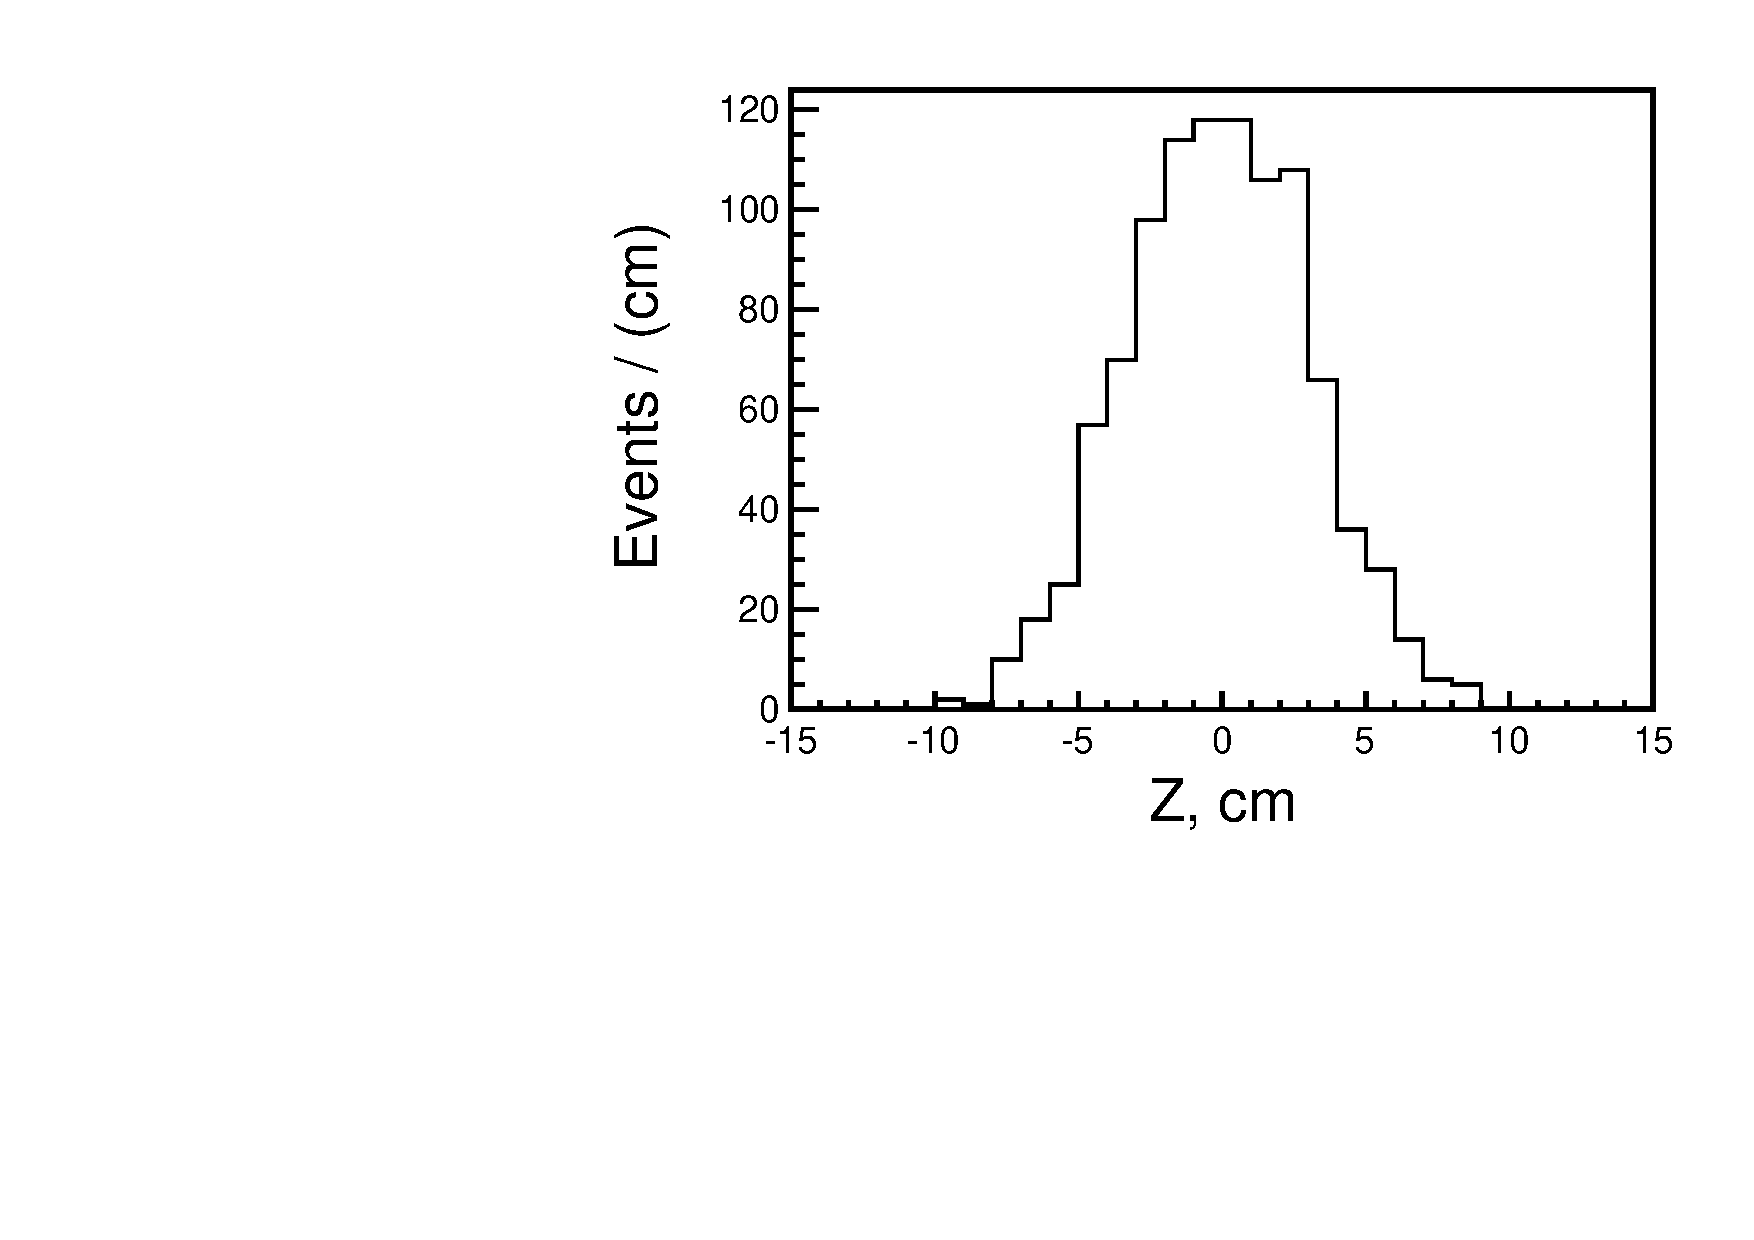
\includegraphics[scale=0.295]{graphs/hVtxZ_v1.pdf}}
        \subfigure{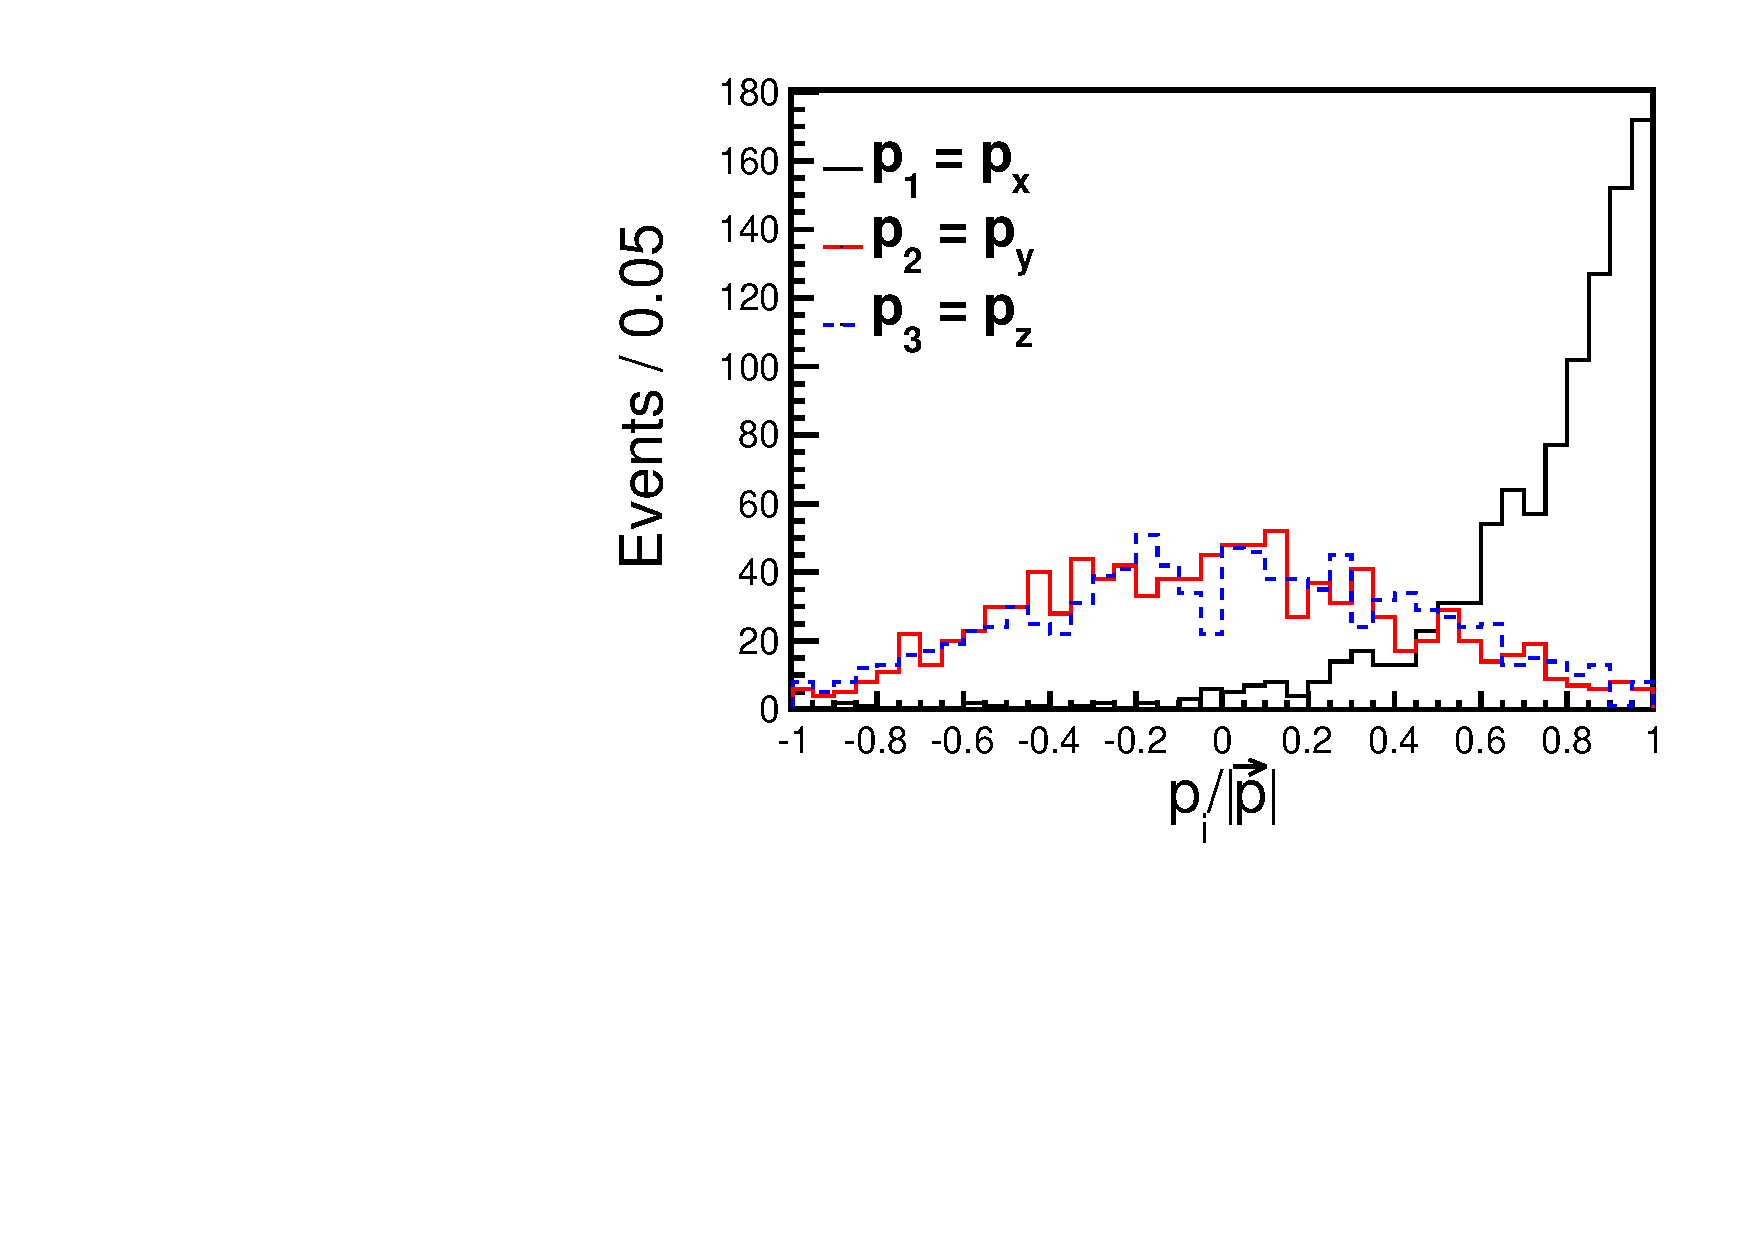
\includegraphics[scale=0.375]{graphs/hDir_pq_1p4.pdf}}
        \subfigure{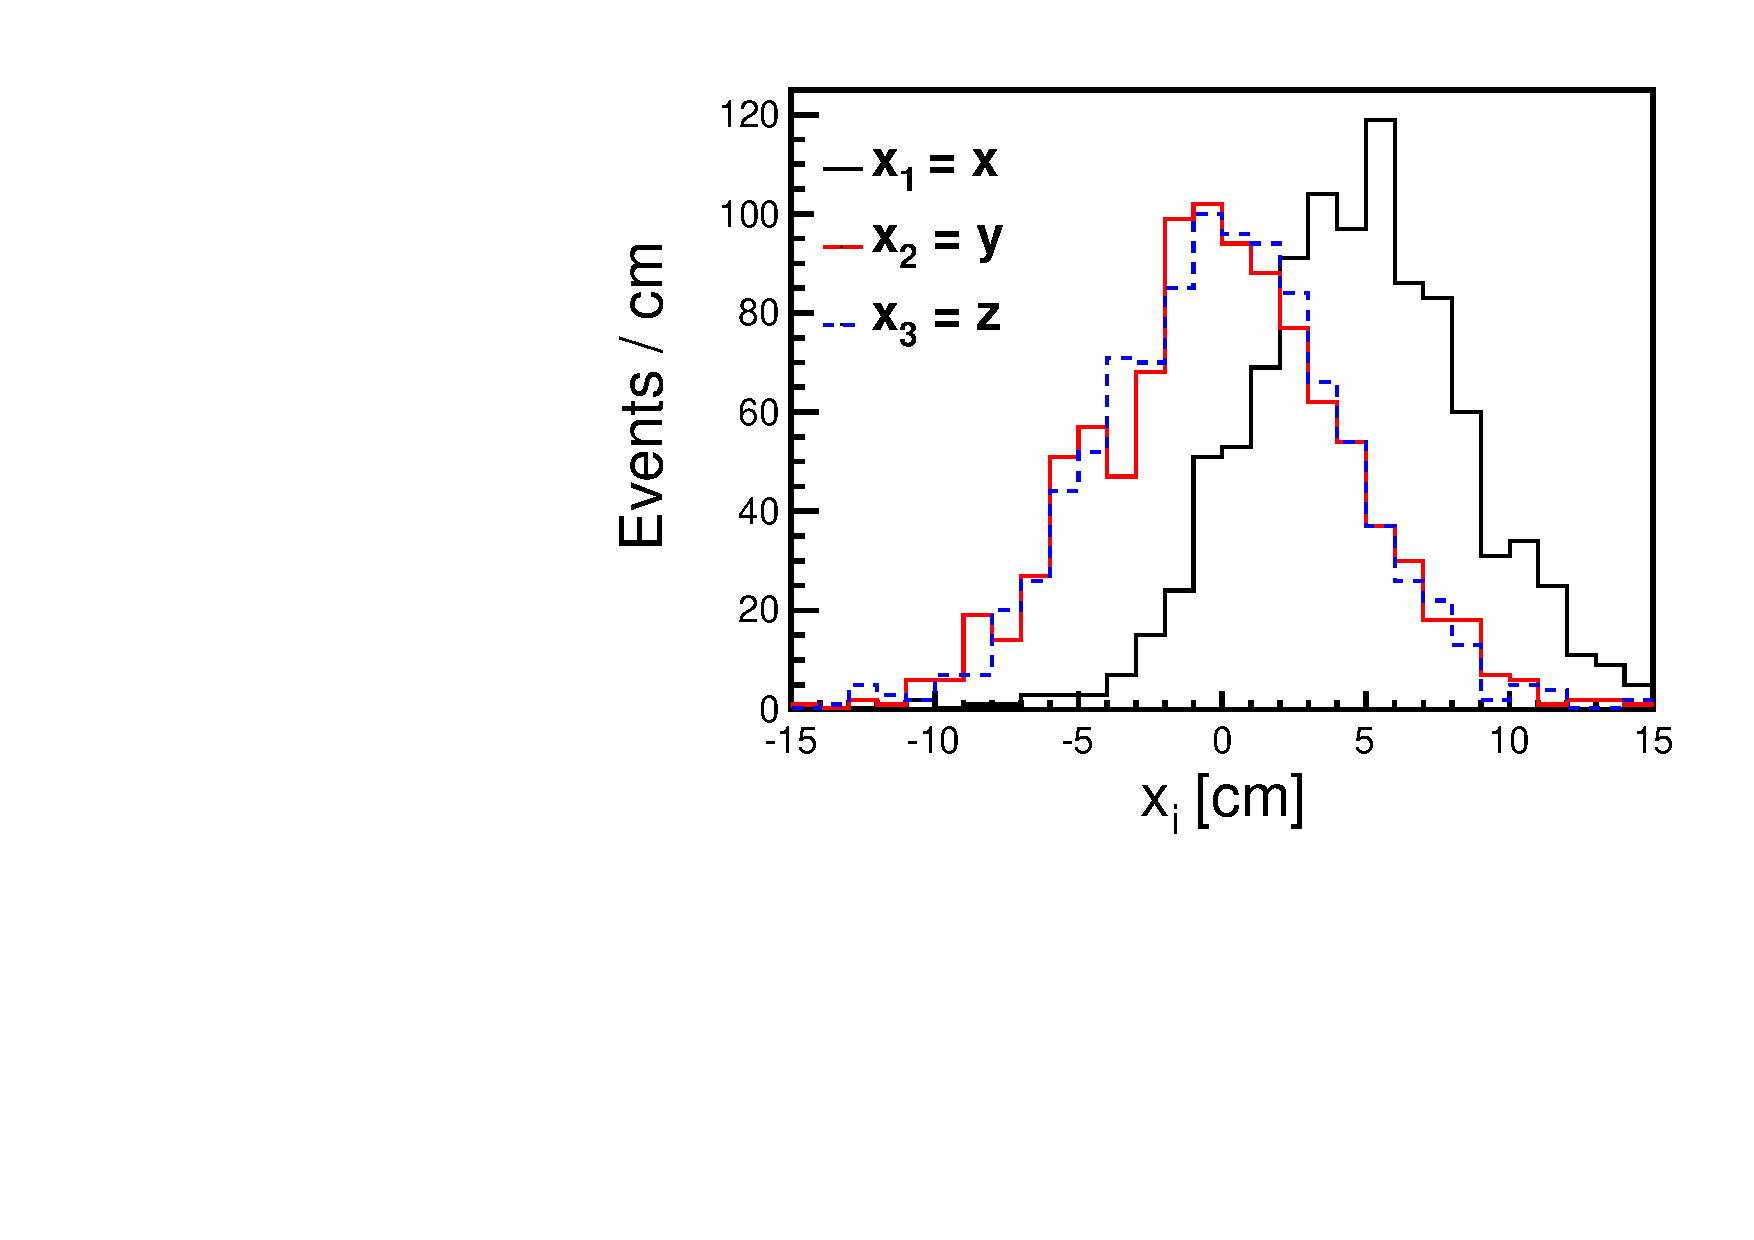
\includegraphics[scale=0.375]{graphs/hVtx_pq_1p4.pdf}}
        \caption[]{(Left) The reconstructed direction,
        $(p_x/|\vec{p}|, p_y/|\vec{p}|,
        p_z/|\vec{p}|)$, for the simulation of 1000 electrons
        (1.4~MeV). In the simulation the electrons are produced along the
        x-axis, $\vec{p}/|\vec{p}|$ = (1,0,0), and originate
        from the center of the 6.5m-radius detector, $\vec{r}$ =
        (0,0,0). Only photons with arrival time of $t<$ 34.0~ns are used
        in the reconstruction. The quantum efficiency of the bialkali
        photocathode is taken into account. (Right) The reconstructed
        vertex position, $(x,y,z)$, for the same simulation. \label{low_energy_reco}}
\end{center}
\end{figure}
\begin{figure}
        \begin{center}
        \includegraphics[scale=0.4]{graphs/hCos_vs_E.pdf}
        \caption[]{Mean cosine of the angle between the true initial electron direction and the reconstructed direction, as a function of the electron energy. For each energy 1000 events have been simulated. Statistical errors are
shown. \label{Edep_angle}}
        \end{center}
\end{figure}

The reconstruction algorithms outlined in section \ref{reconstruction_sec} have also been applied
to the simulations at lower energies. Figure \ref{low_energy_reco} shows the results for 
the lowest simulated electron energy, 1.4~MeV. Most events are still reconstructed well, despite the lower
number of PEs and the decreased $R_{C/S}$. For 1.4~MeV electrons, the distribution RMS values for all three
reconstructed coordinates are smaller than 4.5~cm. The mean cosine of the angle between the true direction
and the reconstructed direction for different energies of the initial electron is shown in figure
\ref{Edep_angle}. The direction reconstruction performance is still promising for energies as low as 1.4~MeV.

\section{Conclusions}
The ability to reconstruct direction in kiloton-scale scintillation
detectors would be a major technological advance for neutrino
experiments, especially those also
searching for neutrino-less double-beta decay. More generally, this technique could
be applied wherever scintillation-based detectors are used. A \GEANT~simulation of a simple spherical detector corresponding to a kiloton
of scintillator shows that timing on the order of 0.1~ns is required
to separate the directional Cherenkov light from the more abundant
scintillation light. The separation can be improved using
photodetectors with more red sensitivity and liquid scintillators with
a more narrow emission spectrum shifted to shorter
wavelengths. Furthermore, simple reconstruction algorithms adapted
from those for water Cherenkov detectors are able to reliably
reconstruct the position and direction of electrons with energies in the few MeV range.
More detailed simulation and advanced reconstruction algorithms will need
to be developed to move to more complicated event
topography, such as those in neutrino-less double-beta decay, but the technique already
appears promising.


\acknowledgments
The authors thank Andrew Blake at University of Cambridge for his work
authoring the WCSimAnalysis code. The authors thank the neutrino
reconstruction group at Iowa State, particularly Mayly Sanchez, Ioana
Anghel, and Tian Xin, for their continued work in developing the
WCSimAnalaysis algorithms and for their insights and expertise
regarding issues related to Cherenkov reconstruction with
fast-timing. The authors also thank Micheal Smy for his development of
the quadruplet-based vertex-finding method. L. Winslow would like to
thank Janet Conrad for many useful discussion on the topic, and
Katsushi Arisaka for discussions on the possible reach of traditional PMTs
and the characteristics of HPDs. C. Aberle and L. Winslow are
supported by funds from University of California Los Angeles. The work
at the University of Chicago is partially supported by DOE
contract DE-SC0008172 and NSF grant PHY-1066014. Matthew Wetstein gratefully
acknowledges support by the Grainger Foundation.

\newpage

\bibliographystyle{JHEP}
\bibliography{DirectionBibliography} 

\end{document}
